\documentclass[utf8, xcolor=dvipsnames]{beamer}
% \usetheme{Frankfurt} % Boadilla - Ilmenau

\usepackage{graphicx}
\usepackage{setspace}
\usepackage{csquotes}
\usepackage{changepage}
\usepackage{color}
\usepackage[colorlinks = TRUE, allcolors = blue]{hyperref}
% \useinnertheme{rectangles}
\usepackage{tikz}
\usetikzlibrary{graphs}
\usetikzlibrary{decorations.pathreplacing}

% \setbeamercovered{transparent}
\setbeamercolor{title}{bg=Blue, fg=white}
\setbeamercolor{title_int}{bg=white, fg=Blue}
\setbeamertemplate{navigation symbols}{}
\setbeamertemplate{itemize items}[circle]
\setbeamertemplate{blocks}[default]
\setbeamertemplate{headline}[default]
\setbeamertemplate{section in head}{}
\setbeamertemplate{subsection in head}{}
\setbeamercolor{section in foot}{fg=Blue, bg=white}
\setbeamercolor{subsection in foot}{fg=Blue, bg=white}
\setbeamercolor{frametitle}{fg=Blue, bg=white}
\setbeamercolor{footlinecolor}{bg=white,fg=Blue}
\useoutertheme[compress]{miniframes}

\makeatother
\setbeamertemplate{footline}
{%
  \leavevmode%
  \hbox{
  \begin{beamercolorbox}[wd=\paperwidth,ht=2.5ex,dp=1.125ex,leftskip=.3cm,rightskip=.3cm plus1fil]{footlinecolor}%
    \usebeamerfont{author in head/foot}
    \insertshorttitle\hfill\insertshortauthor\hfill\insertshortdate\hfill\insertframenumber/\inserttotalframenumber
  \end{beamercolorbox}}%
  \vskip0pt%
}
\setbeamertemplate{headline}[default]
{%
    \def\beamer@entrycode{\vspace*{0pt}}
}
\makeatletter

\title[Civil wars]{Civil wars}
\author[Francisco Villamil]{Francisco Villamil}
\date[UC3M / Fall 2022]{War, peace, and political violence\\Fall 2022\\Universidad Carlos III de Madrid}

\begin{document}


\begin{frame}
  \titlepage
\end{frame}


% ----------------------------------------------------
\begin{frame}
\frametitle{Civil wars}
\centering

\includegraphics[width = \textwidth]{img/amecw}

American Civil War

\end{frame}
% ----------------------------------------------------

% ----------------------------------------------------
\begin{frame}
\frametitle{Civil wars}
\centering

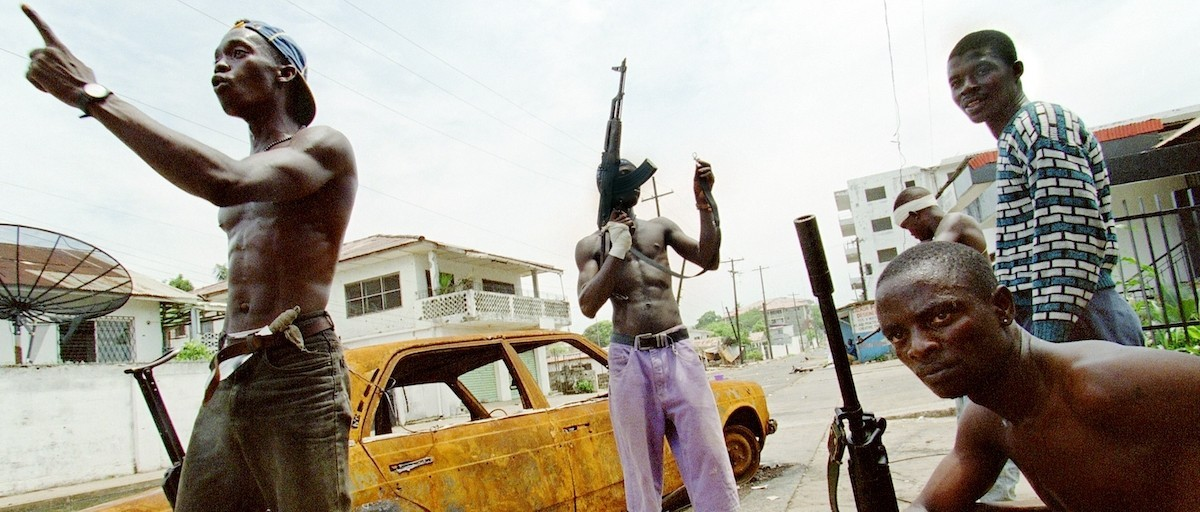
\includegraphics[width = \textwidth]{img/liberia}

Liberian Civil War

\end{frame}
% ----------------------------------------------------

% ----------------------------------------------------
\begin{frame}
\frametitle{Civil wars}
\centering

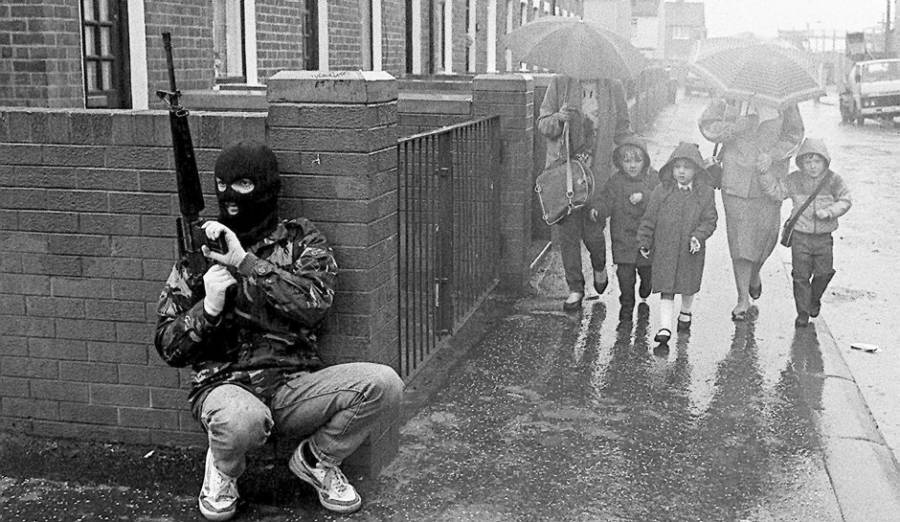
\includegraphics[width = \textwidth]{img/troubles}

Troubles, Northern Ireland

\end{frame}
% ----------------------------------------------------

% ----------------------------------------------------
\begin{frame}
\frametitle{Civil wars}
\centering

\begin{minipage}{0.49\textwidth}\centering
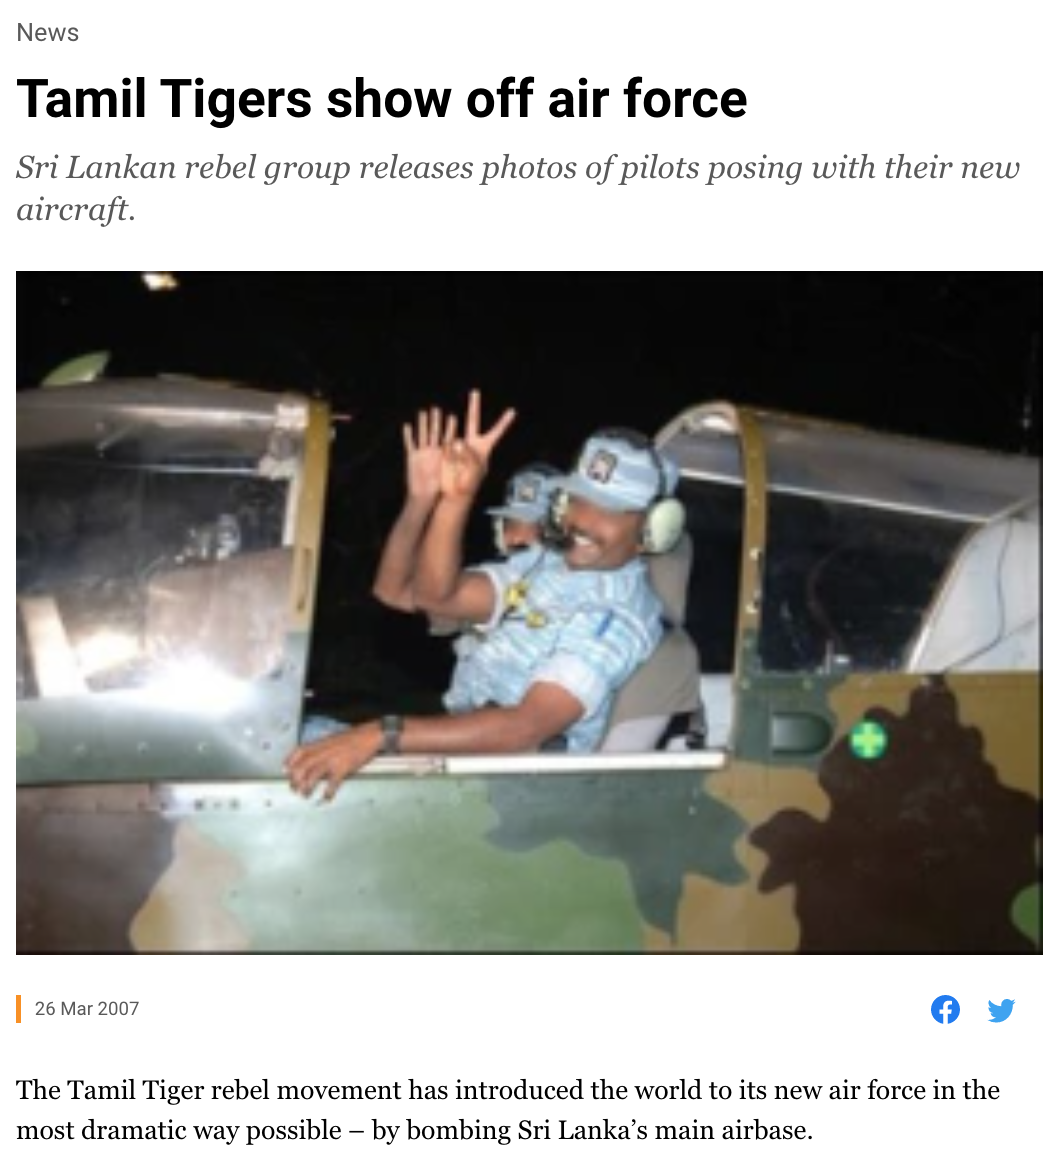
\includegraphics[width = \textwidth]{img/tigers}
\end{minipage}\hfill
\begin{minipage}{0.49\textwidth}\centering
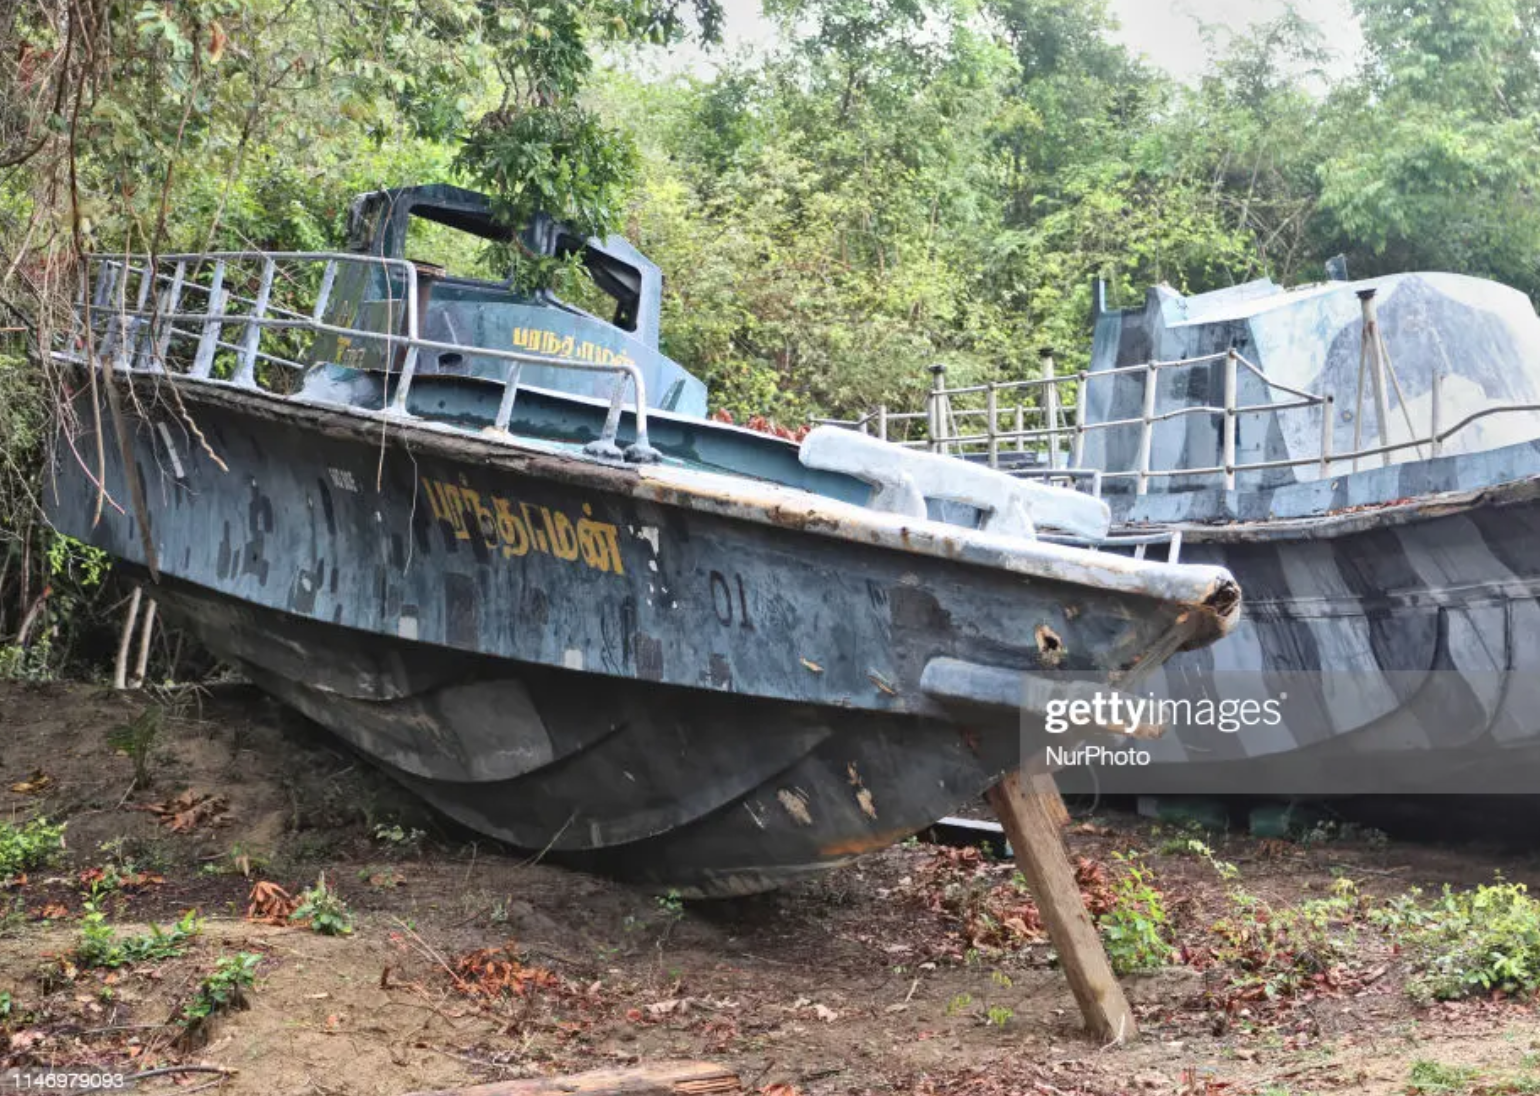
\includegraphics[width = \textwidth]{img/tigersnavy}
\end{minipage}

Sri Lankan war

\end{frame}
% ----------------------------------------------------

% ----------------------------------------------------
\begin{frame}
\frametitle{Civil Wars}
\centering

\begin{minipage}{0.49\textwidth}\centering
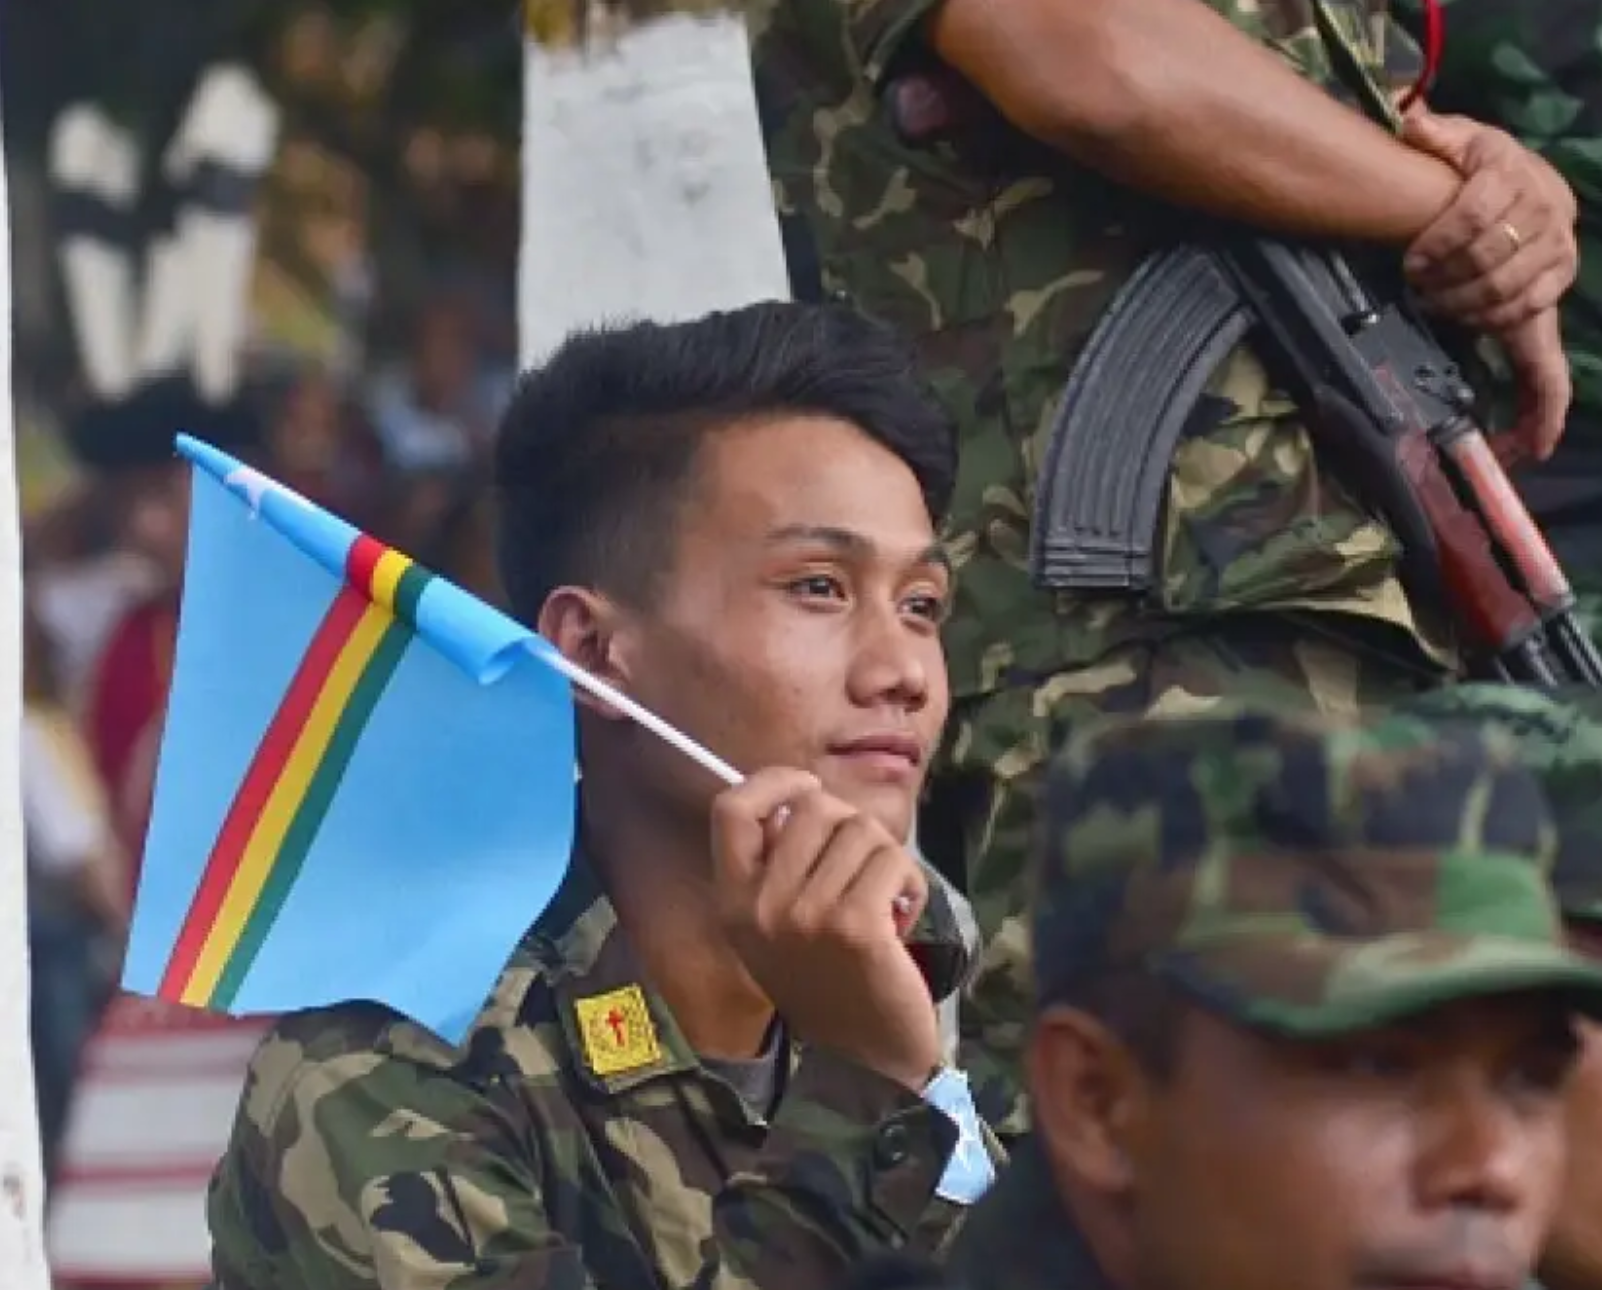
\includegraphics[width = \textwidth]{img/naga1}
\end{minipage}\hfill
\begin{minipage}{0.49\textwidth}\centering
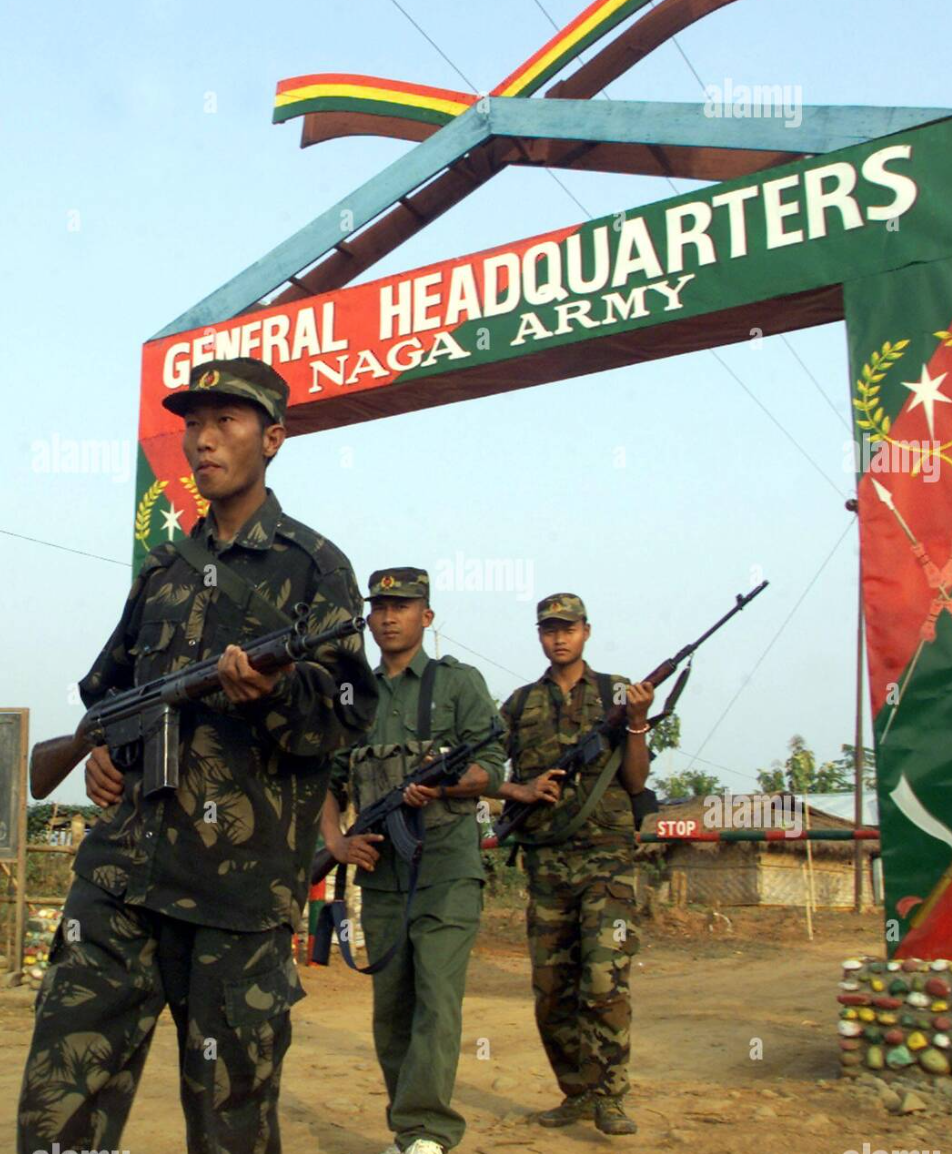
\includegraphics[width = \textwidth]{img/naga2}
\end{minipage}

Nagaland conflict, India

\end{frame}
% ----------------------------------------------------

% ----------------------------------------------------
\begin{frame}
\frametitle{Civil wars}
\centering

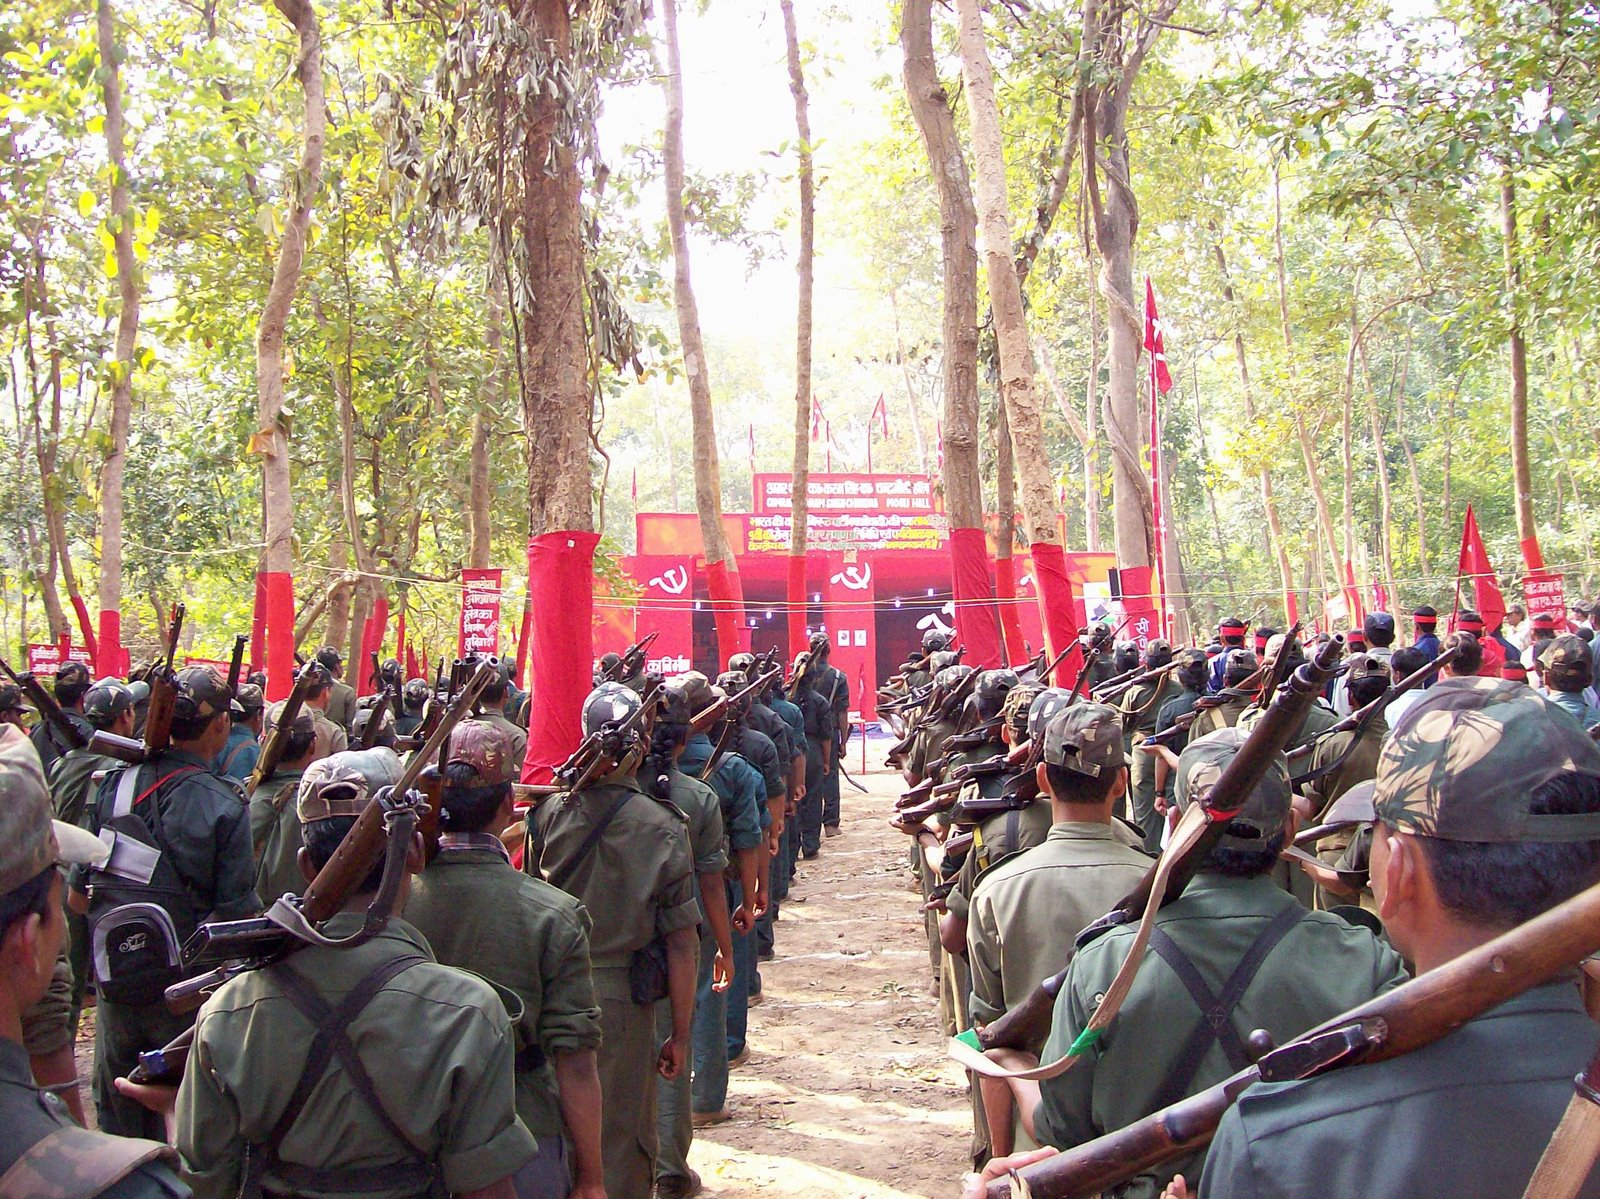
\includegraphics[width = 0.8\textwidth]{img/naxalites}

Naxalites, India

\end{frame}
% ----------------------------------------------------

% ----------------------------------------------------
\begin{frame}
\frametitle{Civil wars}
\centering

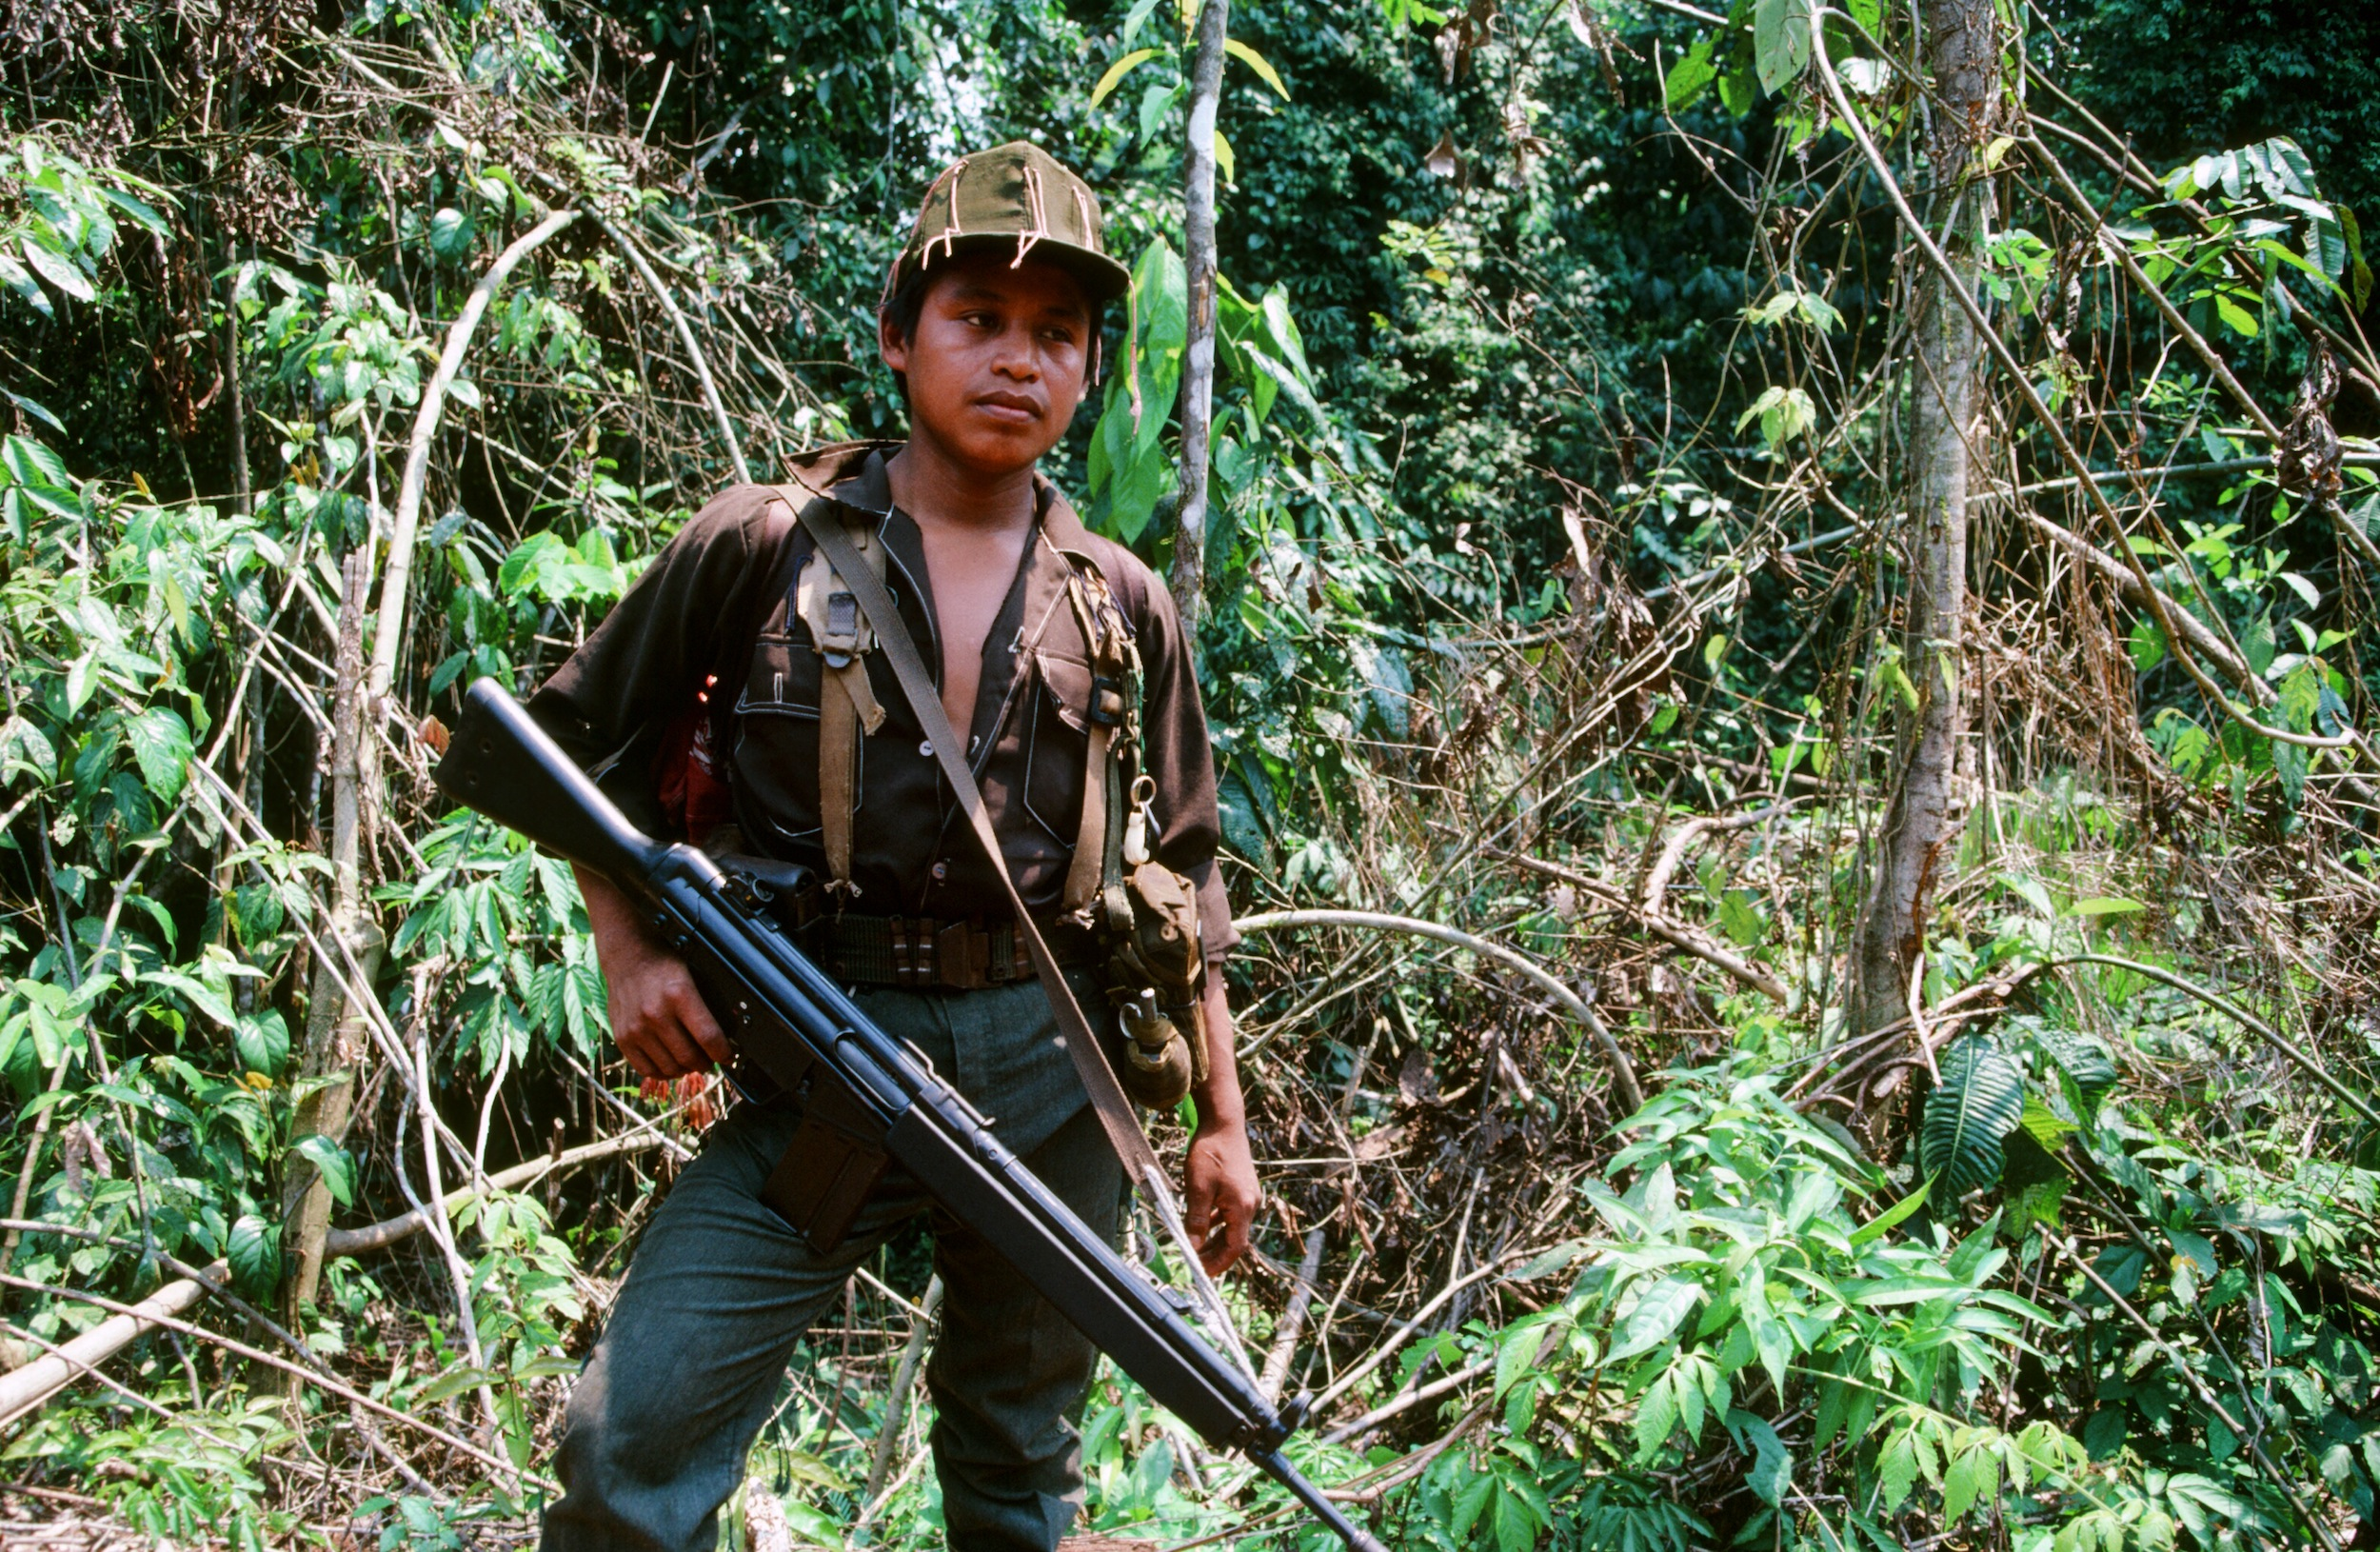
\includegraphics[width = 0.9\textwidth]{img/ixcan1988}

Guatemala

\end{frame}
% ----------------------------------------------------


% ----------------------------------------------------
\begin{frame}
\frametitle{So what is a civil war?}
\centering

\begin{itemize}
  \item What do all these have in common? And differences?
\end{itemize}

\end{frame}
% ----------------------------------------------------

% ----------------------------------------------------
\begin{frame}
\frametitle{So what is a civil war?}
\centering

\begin{itemize}[<+->]
  \item Basic idea: armed conflict \textit{within} a sovereign state, fought between the government and a non-state challenger over opposite claims to sovereignty
  \begin{itemize}
    \item We usually refer to the challengers as \textit{rebel groups}
  \end{itemize}
  \item What is it that they fight over?
  \begin{itemize}
    \item Governmental civil wars: full control of the state
    \item Territorial civil wars: control over one part of the territory
  \end{itemize}
  \item Who is involved?
  \begin{itemize}
    \item Internationalized civil wars: involvement of third-party countries through alliances with local actors
  \end{itemize}
  \item How is the fighting?
  \begin{itemize}
    \item Warfare technology
  \end{itemize}
\end{itemize}

\end{frame}
% ----------------------------------------------------

% ----------------------------------------------------
\begin{frame}
\frametitle{Technologies of rebellion}
\centering

\begin{itemize}[<+->]
  \item Not all rebel groups look the same
  \item Some actually don't even look like rebel groups (or the idea we usually have of them)
  \begin{itemize}
    \item e.g. Confederate States, Franco's Nationalists
  \end{itemize}
  \item Same applies sometimes to the government forces
  \item Concept: technologies of rebellion
  \begin{itemize}
    \item What kind of fighting forces are the rebels capable of launching?
    \item Guerrillas? Conventional armies?
  \end{itemize}
\end{itemize}

\end{frame}
% ----------------------------------------------------

% ----------------------------------------------------
\begin{frame}
\frametitle{Technologies of rebellion}
\centering

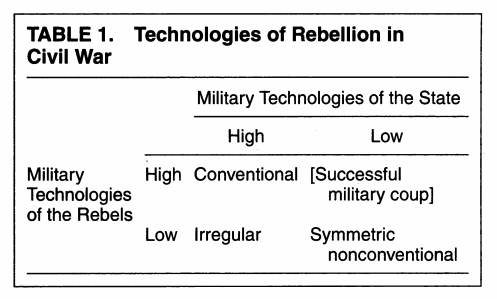
\includegraphics[width = 0.8\textwidth]{img/kalyvas_balcells_tr}\\
{\small Balcells \& Kalyvas (\textit{APSR} 2010)}

\end{frame}
% ----------------------------------------------------

% ----------------------------------------------------
\begin{frame}
\frametitle{Technologies of rebellion}
\centering

\begin{itemize}
  \item Irregular wars
  \begin{itemize}
    \item[] $\approx$ 34\% (1944--2004)
    \item[] (e.g. Nepal, Peru, etc)
  \end{itemize}
  \item Conventional wars
  \begin{itemize}
    \item[] $\approx$ 54\%
    \item[] (e.g. US, Spain, Sri Lanka, Syria)
  \end{itemize}
  \item Symmetric non-conventional
  \begin{itemize}
    \item[] $\approx$ 12\%
    \item[] (Somalia, CAR)
  \end{itemize}
\end{itemize}

\end{frame}
% ----------------------------------------------------

% ----------------------------------------------------
\begin{frame}
\frametitle{What is \textit{not} a civil war?}
\centering

\begin{itemize}
\setbeamercovered{transparent}
  \item<1> It's \textit{not} violence against civilians
  \begin{itemize}
    \item War $\neq$ violence
  \end{itemize}
  \item<2> It's \textit{not} terrorism
  \begin{itemize}
    \item Although terrorism can be used within wars
  \end{itemize}
  \item<3> It's \textit{not} genocide
  \begin{itemize}
    \item Any war involves sustained, bidirectional battle violence
  \end{itemize}
  \item<4> It's \textit{not} non-state violence (e.g. communal riots)
  \begin{itemize}
    \item State/government is always one participant
  \end{itemize}
  \item<5> It's \textit{not} ethnic conflict
  \begin{itemize}
    \item Although there are \textit{ethnic} civil wars (but ethnic conflict also includes ethnic riots, or ethnic violence against civilians)
  \end{itemize}
\end{itemize}

\end{frame}
% ----------------------------------------------------

% ----------------------------------------------------
\begin{frame}
\frametitle{Patterns of conflicts over time}
\centering

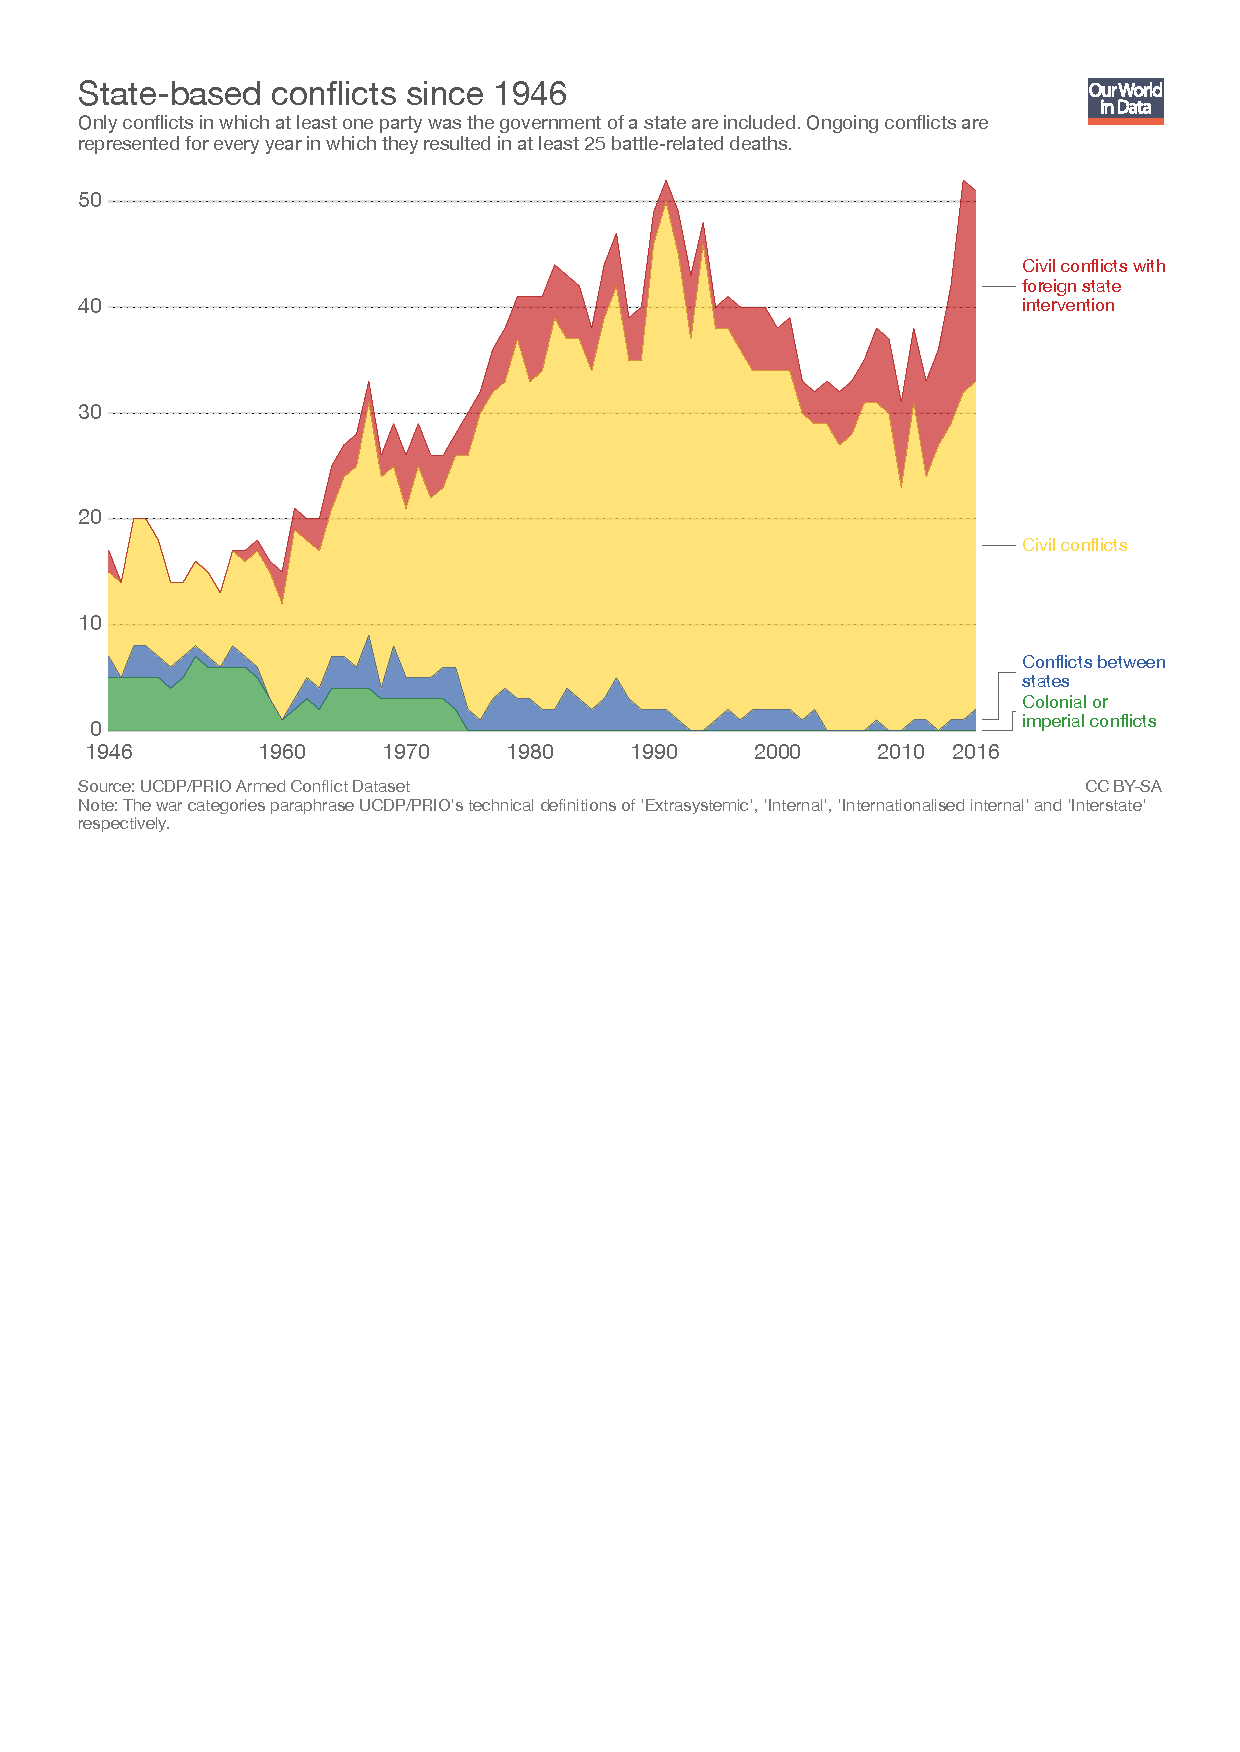
\includegraphics[width = 0.9\textwidth]{img/conflicts_over_time}

{\small \textit{Source:} UCDP-PRIO \& \url{https://ourworldindata.org/}}

\end{frame}
% ----------------------------------------------------

% ----------------------------------------------------
\begin{frame}
\frametitle{Patterns of conflicts over time}
\centering

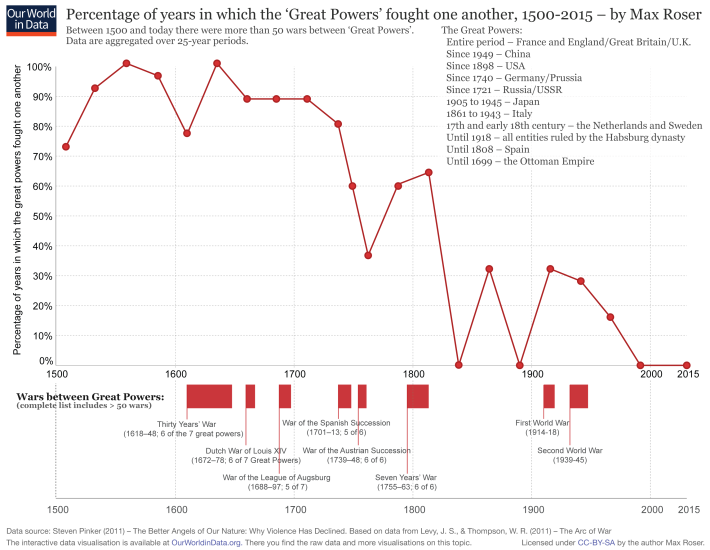
\includegraphics[width = 0.85\textwidth]{img/great_powers_wars}

{\small \textit{Source:} UCDP-PRIO \& \url{https://ourworldindata.org/}}

\end{frame}
% ----------------------------------------------------

% ----------------------------------------------------
\begin{frame}
\frametitle{What do we know about civil wars?}
\centering

\begin{itemize}
  \item<1-> \textbf{Onset of civil wars}
  \begin{itemize}
    \item Why, where and when do they break out?
  \end{itemize}
  \item<2-> Wartime dynamics
  \begin{itemize}
    \item What happens during a civil war? How do we explain wartime violence?
  \end{itemize}
  \item<3-> Termination of civil wars
  \begin{itemize}
    \item How and when do they end?
  \end{itemize}
  \item<4-> Postwar politics
  \begin{itemize}
    \item How do we avoid the relapse of civil wars? What are their consequences?
    \item The `conflict trap'
  \end{itemize}
\end{itemize}

\end{frame}
% ----------------------------------------------------

% ----------------------------------------------------
\begin{frame}
\frametitle{Understanding civil wars}
\centering

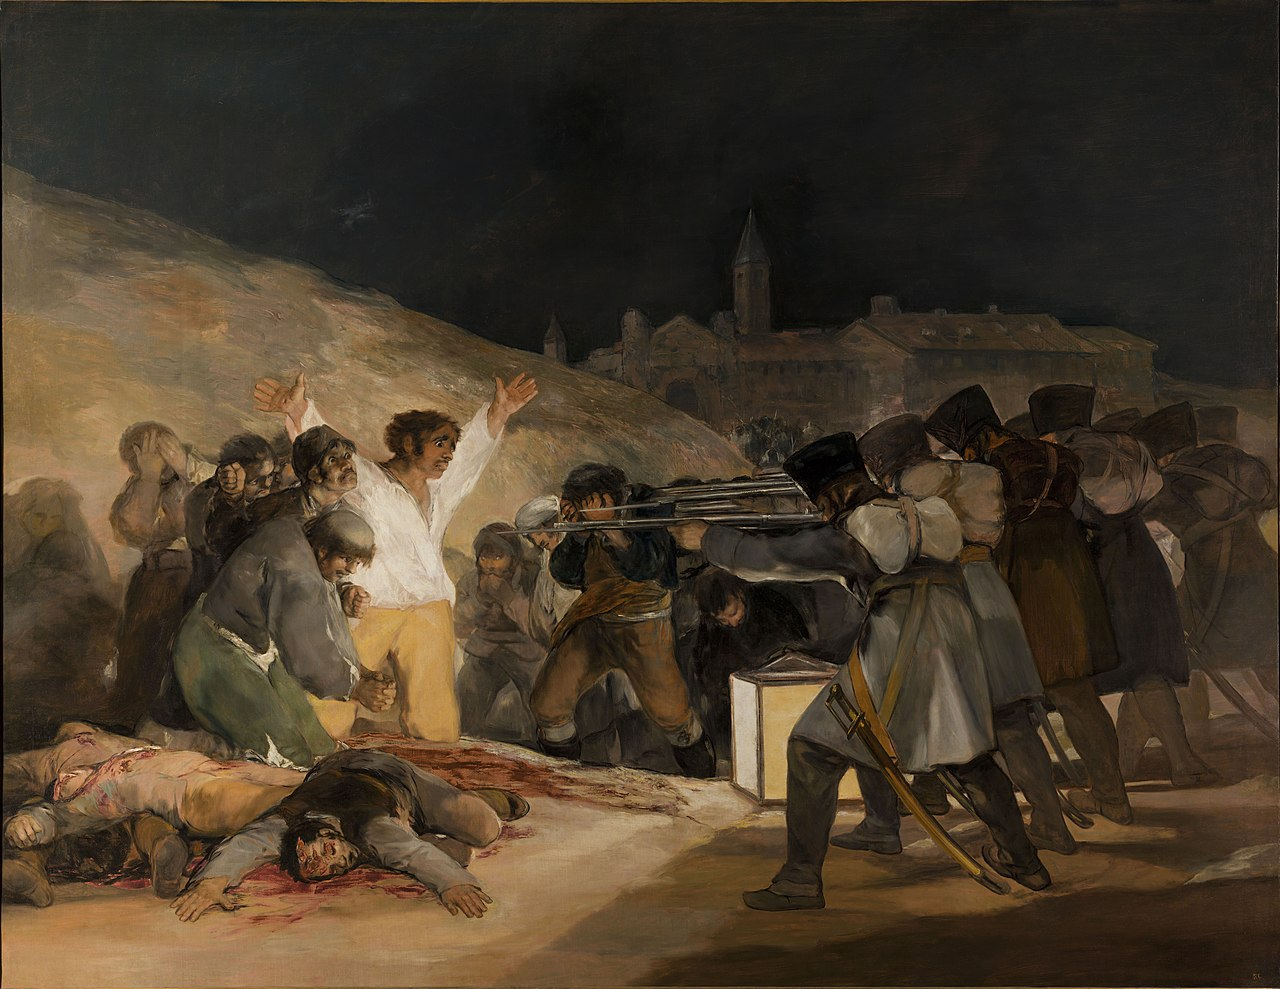
\includegraphics[width = \textwidth]{img/goya}

\textit{Duelo a garrotazos} (Goya, ca. 1820)

\vspace{15pt}

\begin{itemize}
  \item Civil wars were traditionally seen as irrational mass violence
\end{itemize}

\end{frame}
% ----------------------------------------------------

% ----------------------------------------------------
\begin{frame}
\frametitle{Context}
\centering

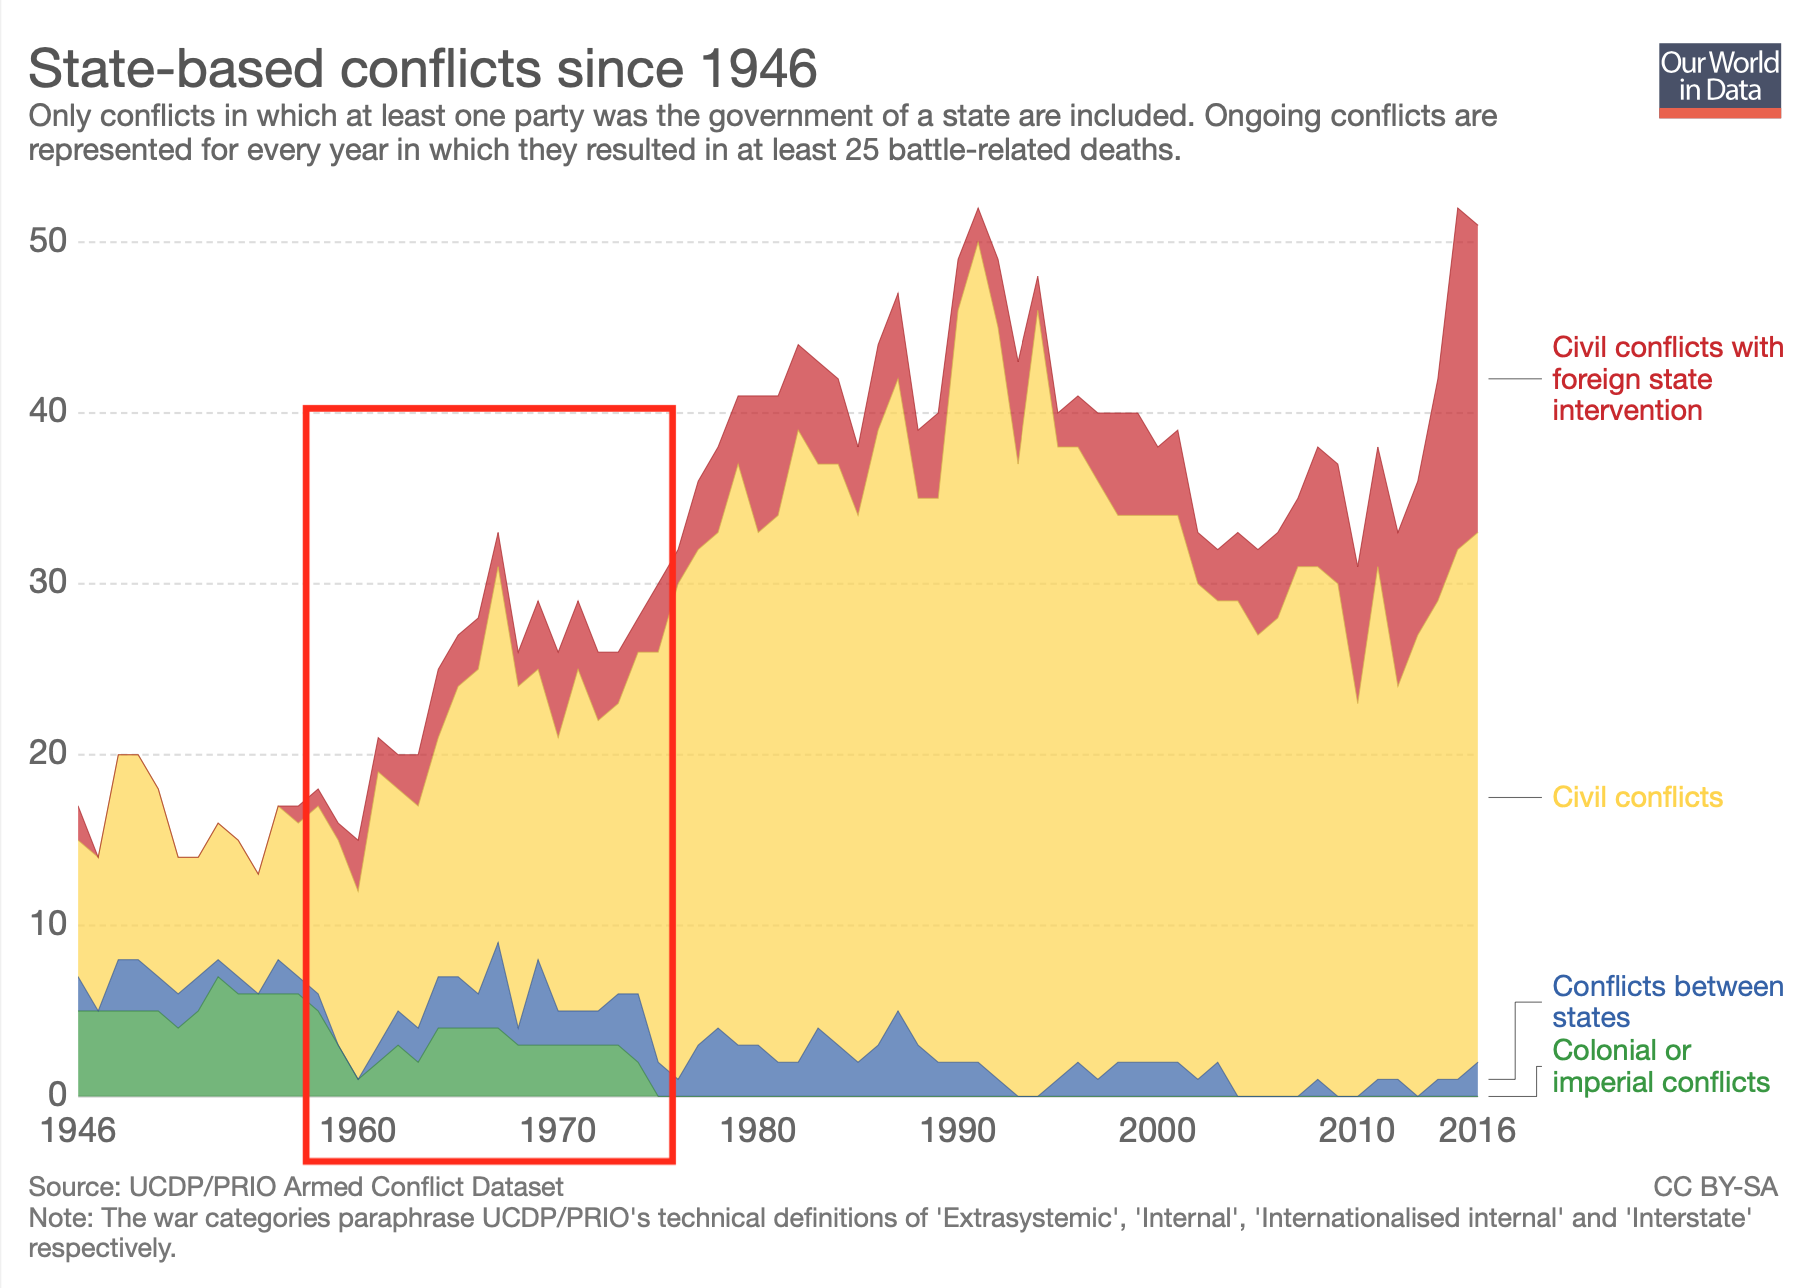
\includegraphics[width = 0.8\textwidth]{img/conflicts_over_time2}

\begin{itemize}
  \item Increase of civil war incidence after the 1960s
\end{itemize}

\end{frame}
% ----------------------------------------------------

% ----------------------------------------------------
\begin{frame}
\frametitle{Context}
\centering

\begin{minipage}{0.49\textwidth}\centering
\begin{itemize}
  \item Role of decolonization from 1960 on
  \item Newly independent countries followed Western-style form of state rule
  \begin{itemize}
    \item Centralized administrations, clear territorial borders (e.g. Organisation of African Unity, Addis Ababa, 1963)
  \end{itemize}
  \item But clear problems of state capacity
\end{itemize}
\end{minipage}\hfill
\begin{minipage}{0.49\textwidth}\centering
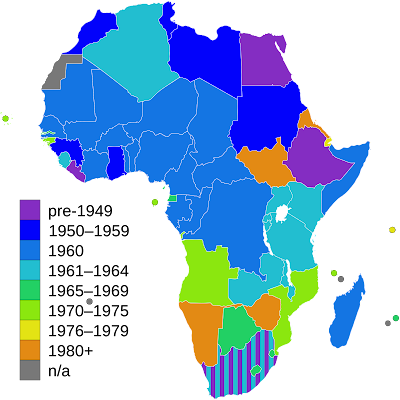
\includegraphics[width = \textwidth]{img/africa_decolonization}\\
Decolonization in Africa
\end{minipage}

\end{frame}
% ----------------------------------------------------

% ----------------------------------------------------
\begin{frame}
\frametitle{Context}
\centering

\begin{minipage}{0.49\textwidth}\centering
\begin{itemize}
  \item Role of decolonization from 1960 on
  \item Newly independent countries followed Western-style form of state rule
  \begin{itemize}
    \item Centralized administrations, clear territorial borders (e.g. Organisation of African Unity, Addis Ababa, 1963)
  \end{itemize}
  \item But clear problems of state capacity
\end{itemize}
\end{minipage}\hfill
\begin{minipage}{0.49\textwidth}\centering
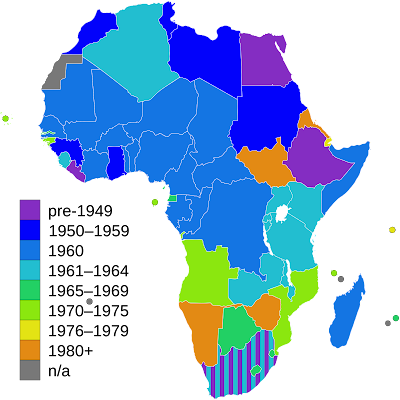
\includegraphics[width = \textwidth]{img/africa_decolonization}\\
Decolonization in Africa
\end{minipage}

\end{frame}
% ----------------------------------------------------

% ----------------------------------------------------
\begin{frame}
\frametitle{Context}
\centering

\begin{minipage}{0.49\textwidth}\centering
\begin{itemize}
  \item Spread of revolutionary insurgencies
  \item Role of ideological global context, Cold War
\end{itemize}
\end{minipage}\hfill
\begin{minipage}{0.49\textwidth}\centering
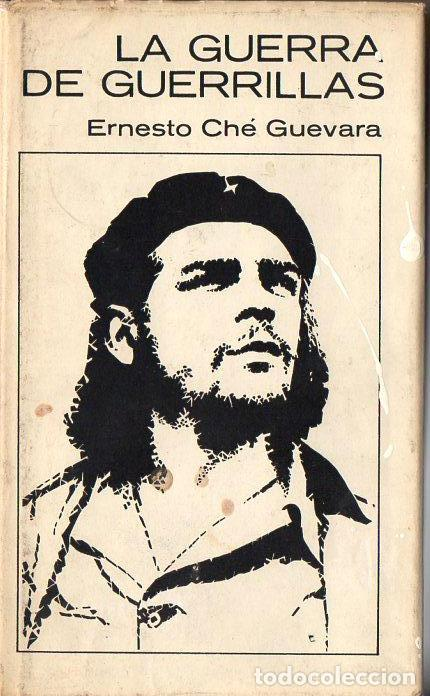
\includegraphics[width = 0.9\textwidth]{img/guevara}
\end{minipage}

\end{frame}
% ----------------------------------------------------

% ----------------------------------------------------
\begin{frame}
\frametitle{Early studies}
\centering

\begin{minipage}{0.59\textwidth}\centering
\begin{itemize}
  \item Early studies on revolutions
  \item Focus on grievances, inequality
  \item That was the prevailing way of studying this before the 1990s
  \item Even if they were \textbf{not} studied as `civil wars,' but as `peasant rebellions' or `social revolutions'
  \begin{itemize}
    \item Mixing onset with outcome, etc
  \end{itemize}
\end{itemize}
\end{minipage}\hfill
\begin{minipage}{0.39\textwidth}\centering
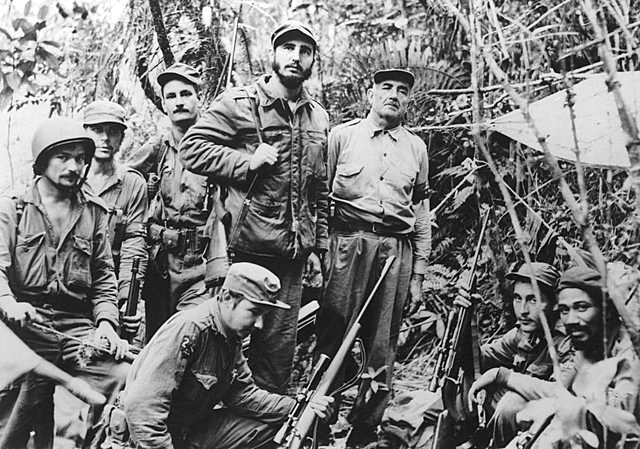
\includegraphics[width = \textwidth]{img/cuban}\\Cuban Revolution
\end{minipage}

\end{frame}
% ----------------------------------------------------

% ----------------------------------------------------
\begin{frame}
\frametitle{Early studies}
\centering

\begin{minipage}{0.59\textwidth}\centering
  \begin{itemize}
    \item Things started to change in the 1990s
    \item The end of the Cold War
    \item Yugoslavia, Rwanda and the role of ethnicity
    \item Ancient hatreds, `clash of civilizations', etc
  \end{itemize}
\end{minipage}\hfill
\begin{minipage}{0.39\textwidth}\centering
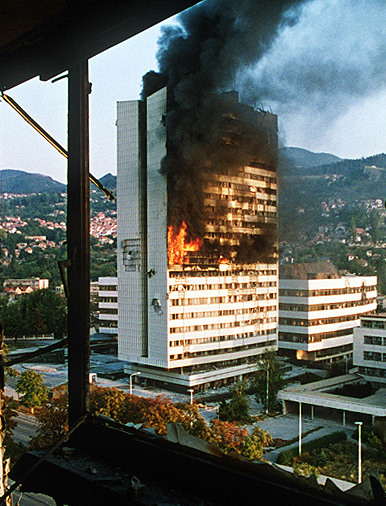
\includegraphics[width = \textwidth]{img/sarajevo}\\Siege of Sarajevo
\end{minipage}

\end{frame}
% ----------------------------------------------------

% ----------------------------------------------------
\begin{frame}
\frametitle{Research on `civil wars'}
\centering

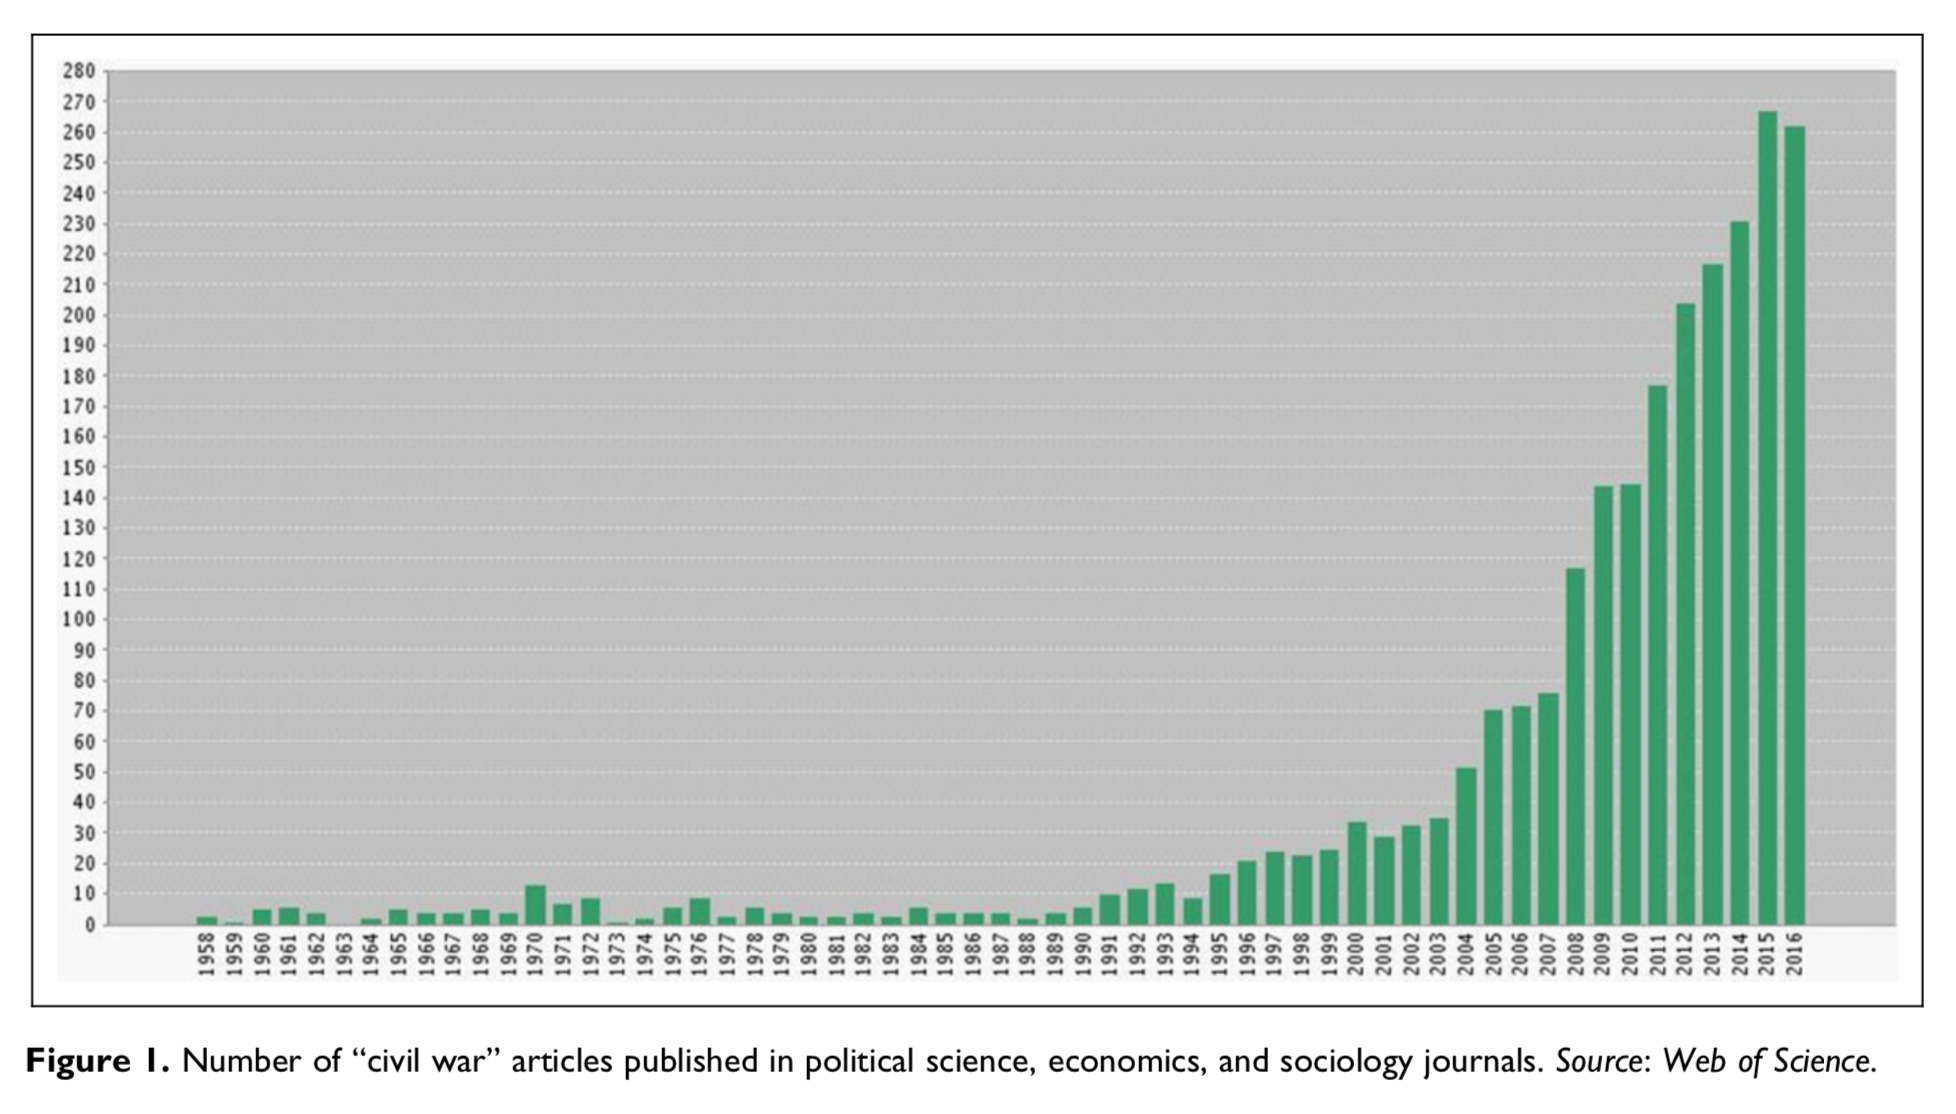
\includegraphics[width = \textwidth]{img/cw_studies}

\end{frame}
% ----------------------------------------------------

% ----------------------------------------------------
\begin{frame}
\frametitle{How it started: the role of development economists}
\centering

\begin{minipage}{0.5\textwidth}\centering
\begin{itemize}
  \item Civil wars as a development problem
  \item What drives civil wars?
  \item First quantitative analyses of CW onset
  \item New explanation: greed
  \begin{itemize}
    \item Greed vs. grievance debate
  \end{itemize}
\end{itemize}
\end{minipage}\hfill
\begin{minipage}{0.5\textwidth}\centering
\frame{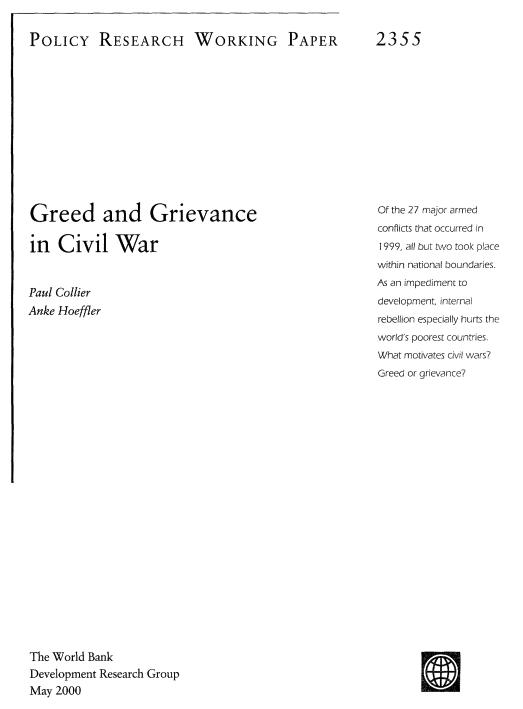
\includegraphics[width = 0.85\textwidth]{img/greed_grievance}}\\
{\small Paul Collier \& Anke Hoeffler (2000)}
\end{minipage}

\end{frame}
% ----------------------------------------------------

% ----------------------------------------------------
\begin{frame}
\frametitle{The \textit{greed} perspective}
\centering

\begin{itemize}[<+->]
  \item Previous studies on revolutions highlighted the role of grievances: peasants rise up because they are oppresed
  \item Collier \& Hoeffler argued that grievances do not explain anything because they are always present
  \item Grievances are just used by \textit{greedy rebels} who think a civil war is a good opportunity to get rich
  \item Microeconomic perspective: civil wars erupt if the the opportunity cost of violence is low (poverty) and the expected gains are high (natural resources \& looting)
\end{itemize}

\end{frame}
% ----------------------------------------------------

% ----------------------------------------------------
\begin{frame}
\frametitle{Empirics in Collier \& Hoeffler model}
\centering

\begin{itemize}
  \item[] Key variables:
  \item Male secondary schooling
  \item Primary commodity exports
  \item Social fractionalization
  \item[]
  \item Analyzing determinants of onset in country-year data
\end{itemize}

\end{frame}
% ----------------------------------------------------

% ----------------------------------------------------
\begin{frame}
\frametitle{}
\centering

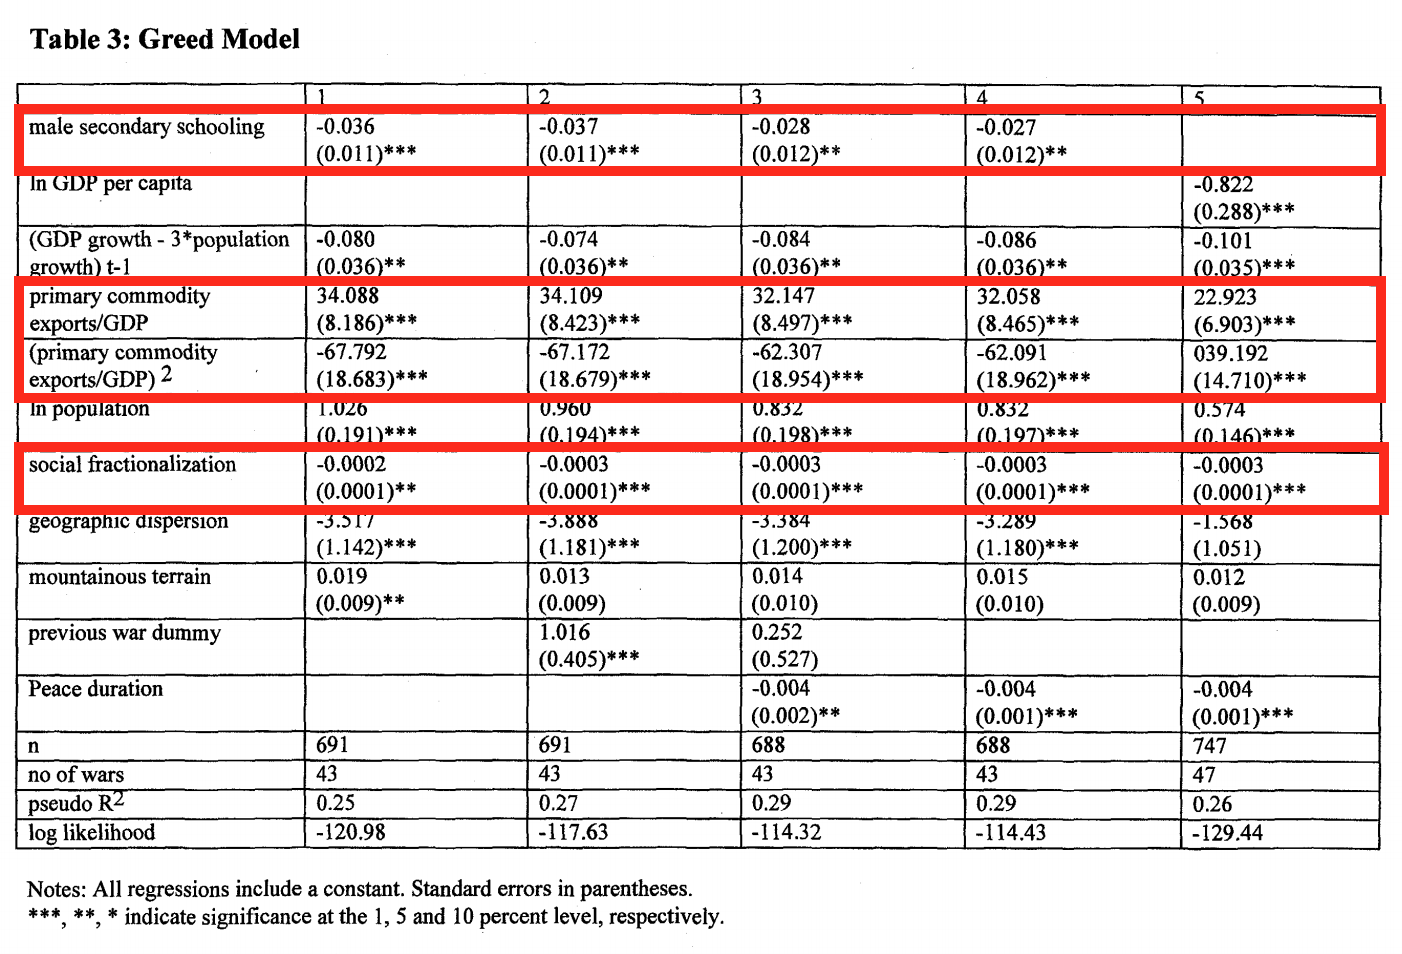
\includegraphics[width = \textwidth]{img/collier_hoeffler_model}

{\small Collier \& Hoeffler (2000)}

\end{frame}
% ----------------------------------------------------

% ----------------------------------------------------
\begin{frame}
\frametitle{The \textit{greed} perspective: context}
\centering

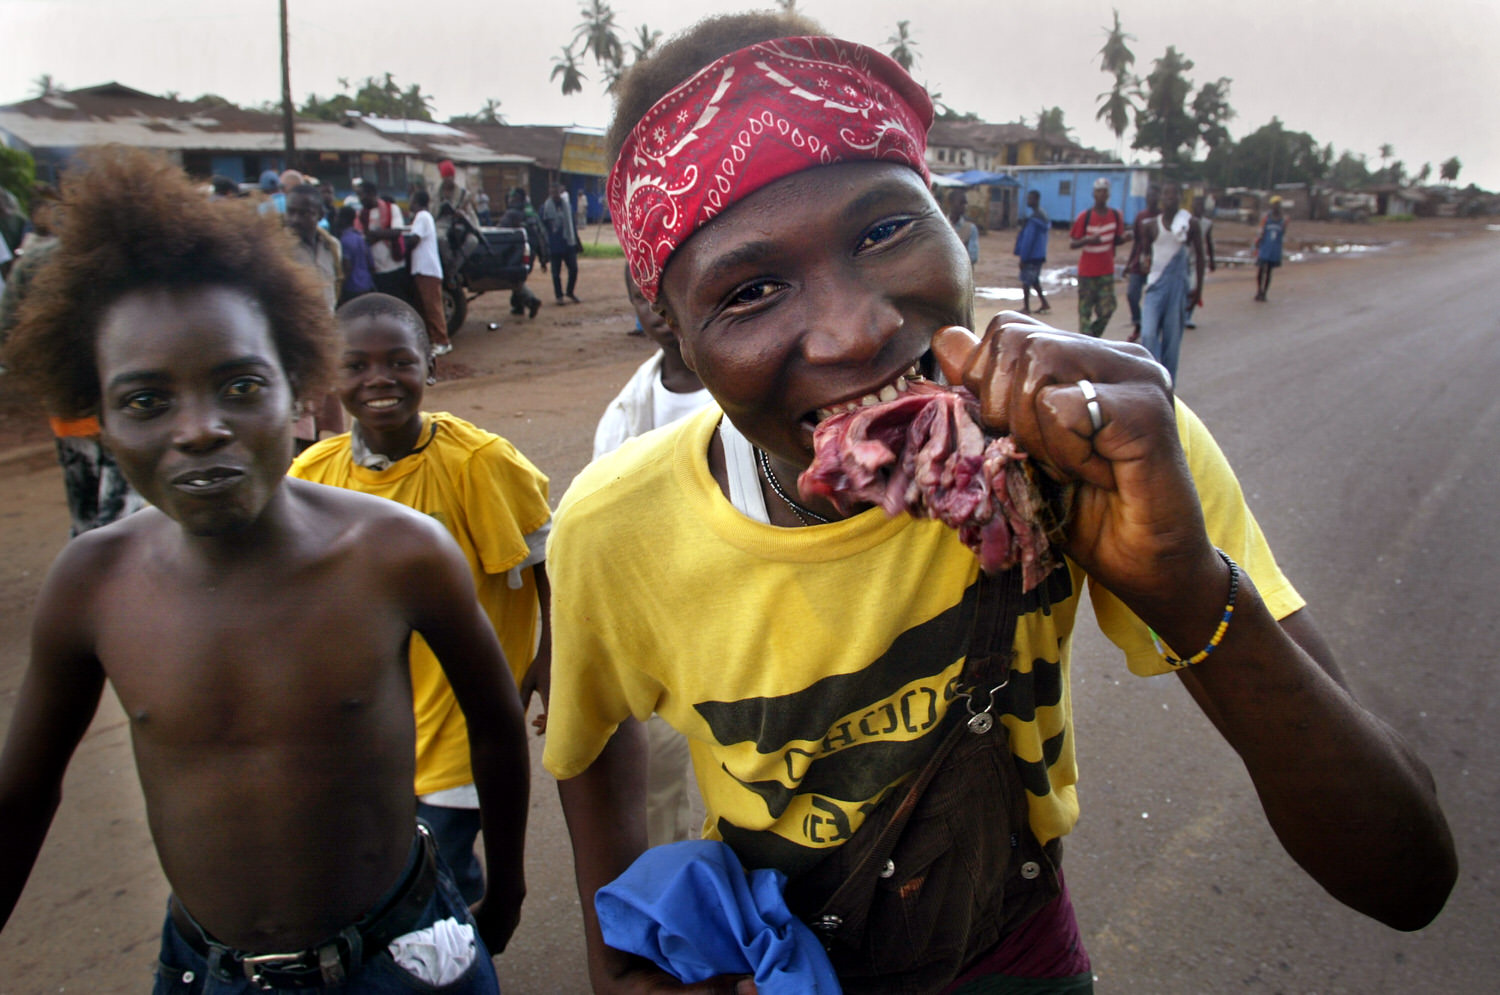
\includegraphics[width = 0.75\textwidth]{img/liberia_curtis}

{\footnotesize Liberian Civil War (Ben Curtis)}\\\vspace{10pt}

\begin{itemize}
  \item End of the Cold War and the big ideologies
  \item New wars, resource-rich countries, warlords
\end{itemize}

\end{frame}
% ----------------------------------------------------

% ----------------------------------------------------
\begin{frame}
\frametitle{In practice}
\centering

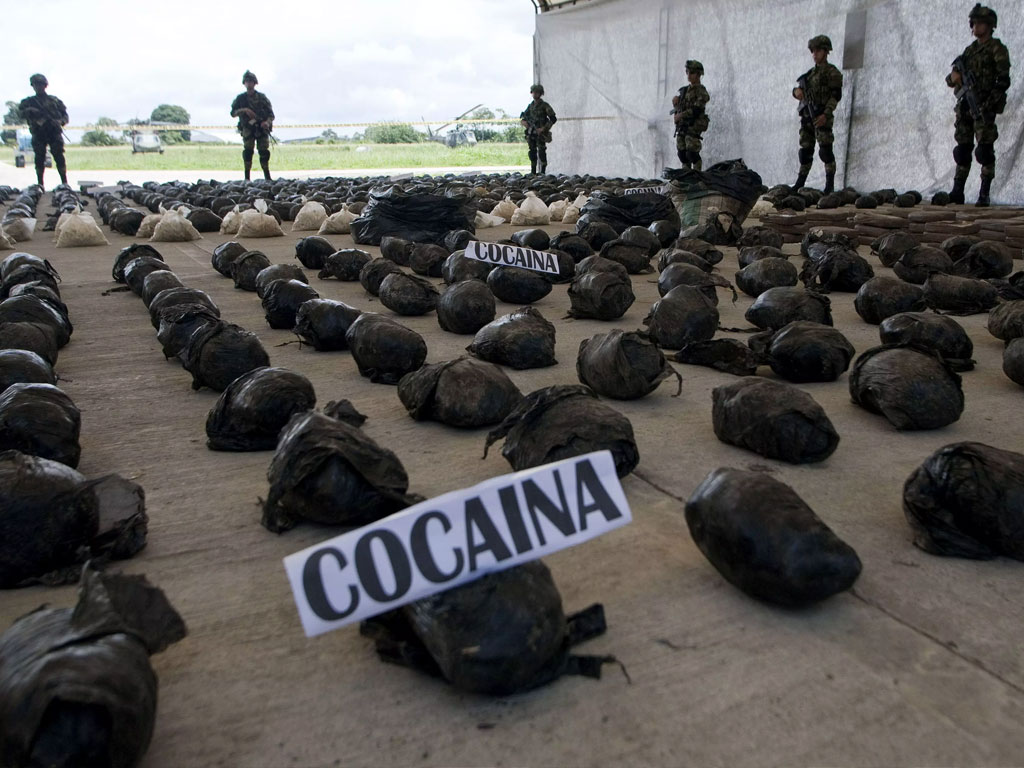
\includegraphics[width = 0.8\textwidth]{img/farc}

FARC and cocaine in Colombia

\end{frame}
% ----------------------------------------------------

% ----------------------------------------------------
\begin{frame}
\frametitle{In practice}
\centering

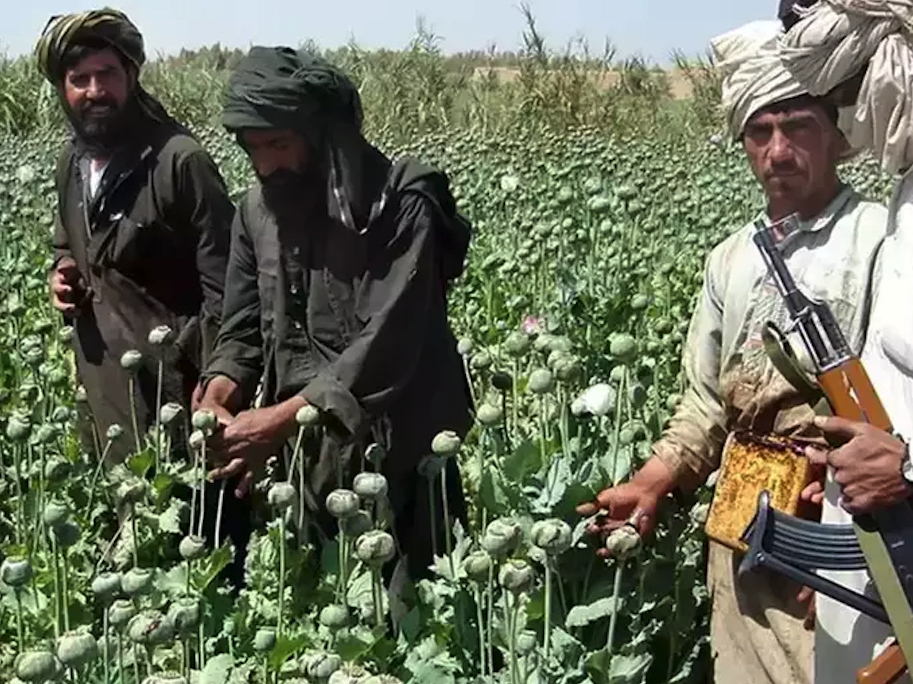
\includegraphics[width = 0.8\textwidth]{img/taliban}

Taliban and opium in Afghanistan

\end{frame}
% ----------------------------------------------------

% ----------------------------------------------------
\begin{frame}
\frametitle{In practice}
\centering

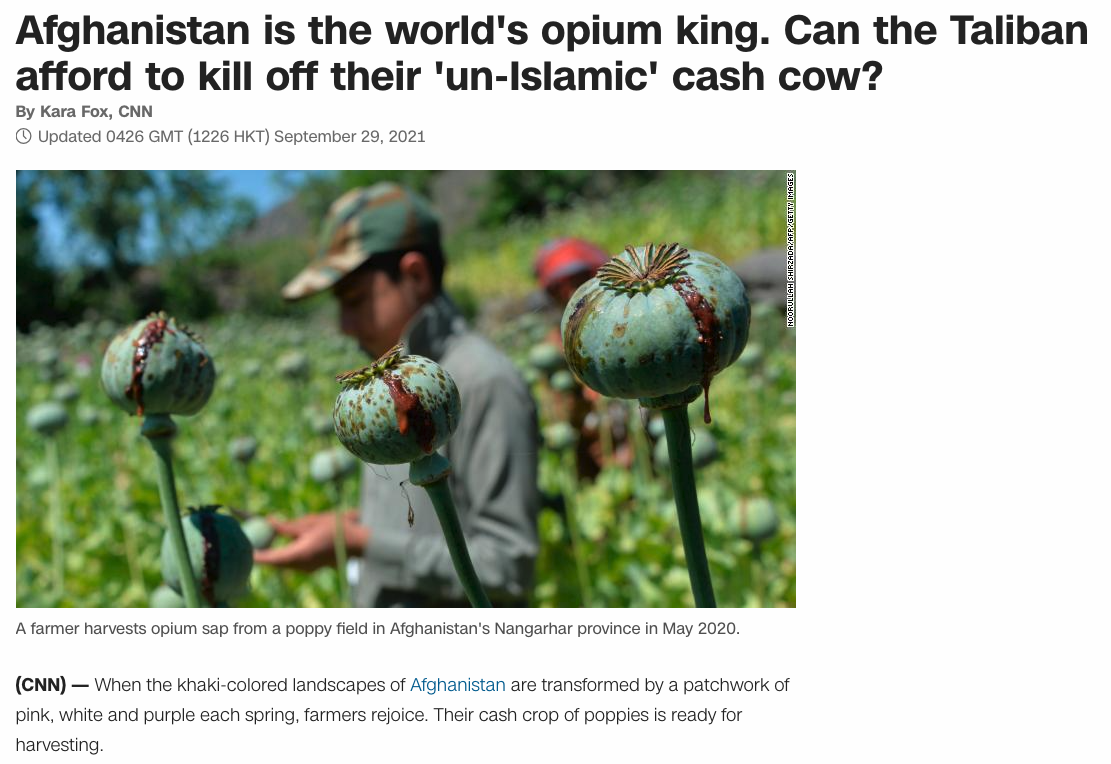
\includegraphics[width = 0.8\textwidth]{img/taliban_cnn}

By the way, how could we explain this? (i.e. Taliban trying to erradicate opium trade after getting power)

\end{frame}
% ----------------------------------------------------

% ----------------------------------------------------
\begin{frame}
\frametitle{Implications}
\centering

\begin{minipage}{0.58\textwidth}\centering
\begin{itemize}
  \item Greed perspective is actually quite common {\small (not only for civil wars)}
  \item Not only about an academic debate on the causes, but with major implications for conflict resolution
  \item Causes of onset $\ineq$ organizational behavior
\end{itemize}
\end{minipage}\hfill
\begin{minipage}{0.40\textwidth}\centering
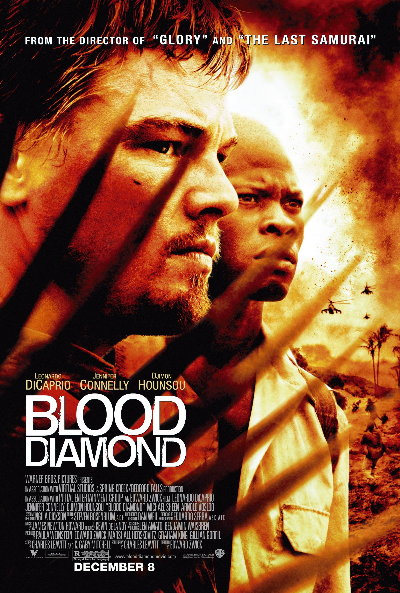
\includegraphics[width = 0.9\textwidth]{img/Blooddiamondposter}
\end{minipage}

\end{frame}
% ----------------------------------------------------

% ----------------------------------------------------
\begin{frame}
\frametitle{Refining \textit{greed} model: opportunity}
\centering

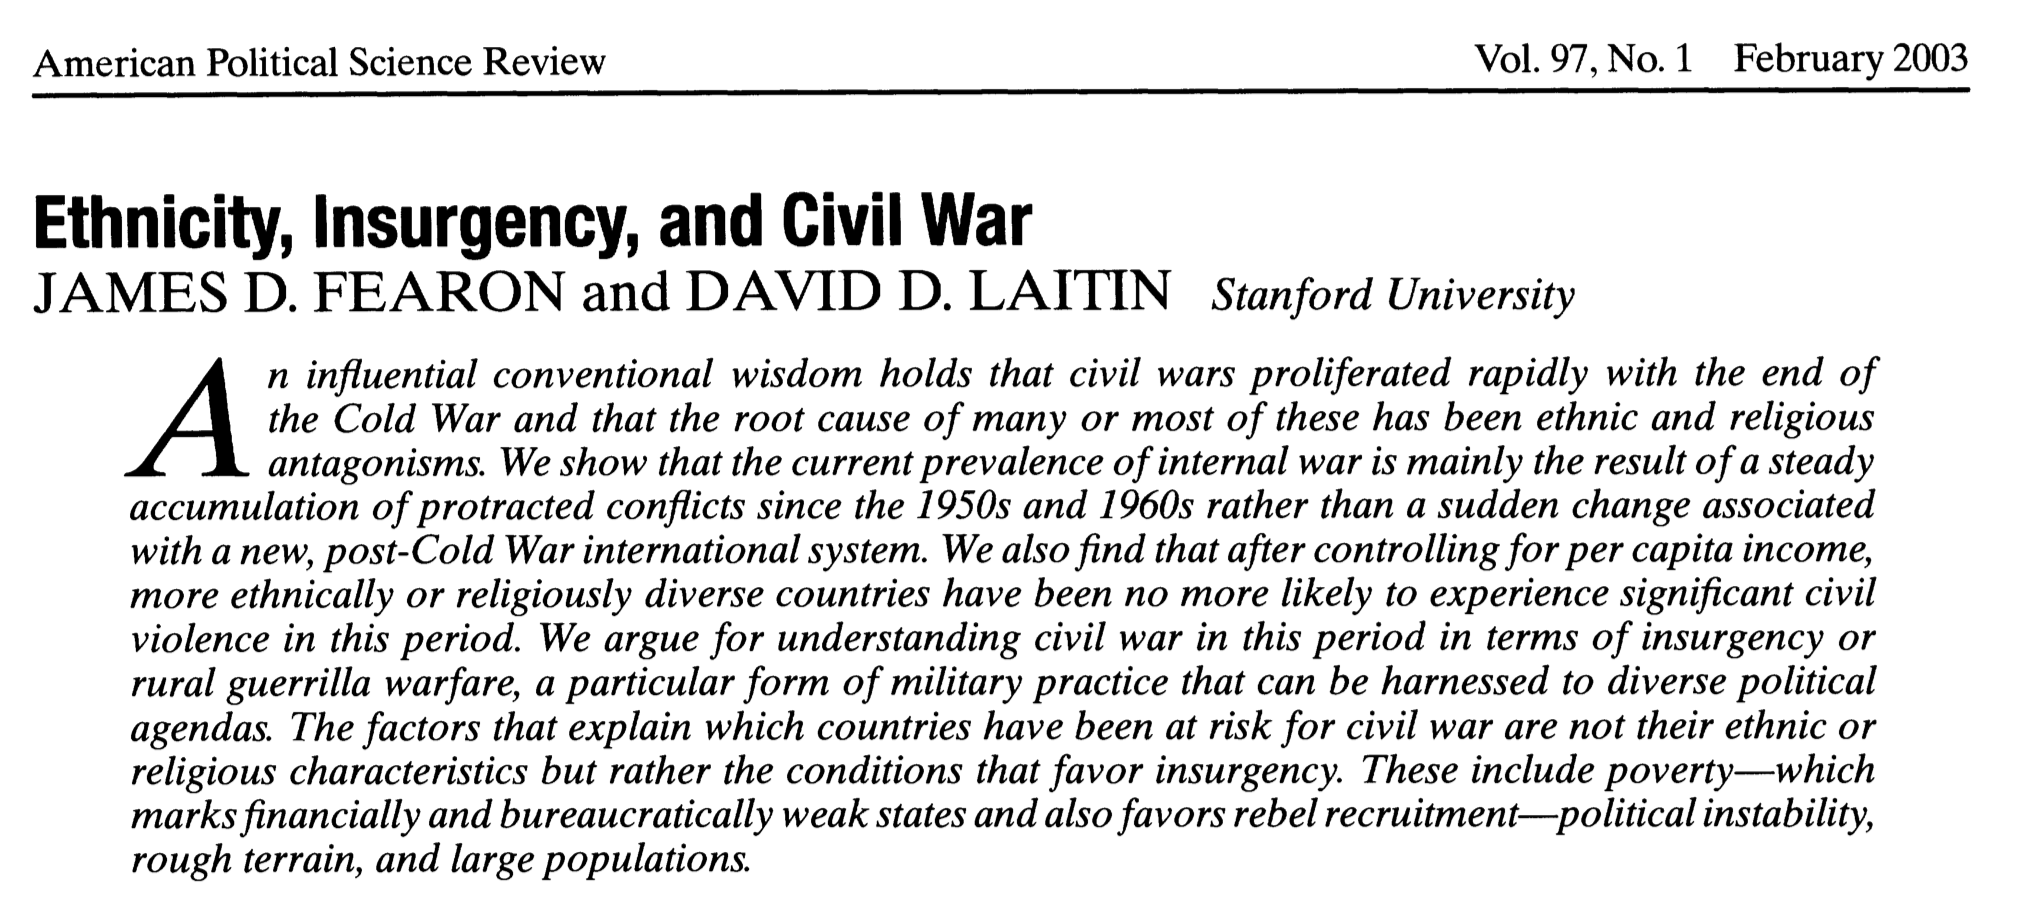
\includegraphics[width = \textwidth]{img/fearon_laitin}

\begin{itemize}
  % \item Fearon \& Laitin (2003) Ethnicity, Insurgency, and Civil War (\textit{American Political Science Review})
  \item Stressing \textit{opportunity} instead of greed
  \item Most influential explanation on civil war
\end{itemize}

\end{frame}
% ----------------------------------------------------

% ----------------------------------------------------
\begin{frame}
\frametitle{Fearon \& Laitin's model of insurgency}
\centering

\begin{itemize}[<+->]
  \item It's not about greedy rebels calculating how to get rich
  \item Civil war erupts when the state is weak (\& up for grabs by political opponents)
  \item Focus on the `technology of insurgency': factors that improve the capacity of rebels to launch an armed conflict using ``small, lighly armed bands practicing guerrilla warfare from rural base areas''
\end{itemize}

\end{frame}
% ----------------------------------------------------

% ----------------------------------------------------
\begin{frame}
\frametitle{Fearon \& Laitin's model of insurgency}
\centering

\begin{itemize}[<+->]
  \item What makes these rural insurgencies more likely?
  \item[-] Poverty
  \begin{itemize}
    \item weak states that do not police as good \& it is easier for the rebels to recruit
  \end{itemize}
  \item[-] Rough terrain
  \begin{itemize}
    \item easier for the rebels to organize, hide from the state (state capacity again)
  \end{itemize}
  \item[-] Political instability
  \begin{itemize}
    \item disorganized center of power, less capacity to control
  \end{itemize}
  \item[-] Large populations
  \begin{itemize}
    \item again, more difficult to control and easier rebel recruitment
  \end{itemize}
  \item Importantly, F\&L \textbf{ruled out} the effect of ethnic or religious divisions
\end{itemize}

\end{frame}
% ----------------------------------------------------

% ----------------------------------------------------
\begin{frame}
\frametitle{Fearon \& Laitin's diagnoses}
\centering

\begin{itemize}[<+->]
  \item Focus on the `\textbf{resource curse}': countries that depend on natural resources are more likely to suffer insurgencies and conflict
  \item Collier \& Hoeffler's greed model: they are easy to loot
  \item Fearon \& Laitin's opportunity model: resource-rich countries don't need to develop tax extraction and public services, leading to bad governance and weak institutions
  \item Particularly much worse in countries with rough terrain and peripherical regions
  \begin{itemize}
    \item Remember Tilly's model of state creation?
    \item If you have oil or diamonds, no need to develop state structures for taxation
  \end{itemize}
\end{itemize}

\end{frame}
% ----------------------------------------------------

% ----------------------------------------------------
\begin{frame}
\frametitle{Fearon \& Laitin's diagnoses}
\centering

\begin{minipage}{0.49\textwidth}\centering
\begin{itemize}[<+->]
  \item So that's the main reason why we observed the post-1960 increase in civil war
  \item \textbf{Not} because of grievances related to the decolonization process, but because these states were `half-baked'
  \item (Same argument applies to Latin America, according to them)
\end{itemize}
\end{minipage}\hfill
\begin{minipage}{0.49\textwidth}\centering
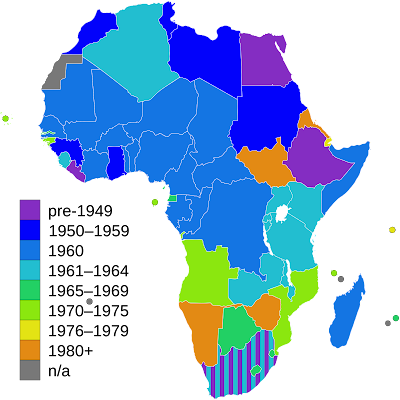
\includegraphics[width = \textwidth]{img/africa_decolonization}\\
Decolonization in Africa
\end{minipage}

\end{frame}
% ----------------------------------------------------

% ----------------------------------------------------
\begin{frame}
\frametitle{So what happened in 1990? (according to F\&L)}
\centering

\begin{itemize}[<+->]
  \item Civil war incidence \textit{appeared} to rise markedly after the end of the Cold War
  \item Previous explanations on the role of the international system or the rise of multi-ethnic countries
  \item Fearon \& Laitin: it's not new wars but the consequence of many protracted conflicts that have not still ended, brought about by the new weak states created in the decolonization waves of the 1950s and 1970s
  \item So we should focus on the technology of insurgency, the \textit{domestic} conditions that favor rebellion, and not on cultural, ethnic, or religious differences
\end{itemize}

\end{frame}
% ----------------------------------------------------

% ----------------------------------------------------
\begin{frame}
\frametitle{}
\centering

\textbf{Part 2}

\end{frame}
% ----------------------------------------------------

% ----------------------------------------------------
\begin{frame}
\frametitle{Greed \& opportunity}
\centering

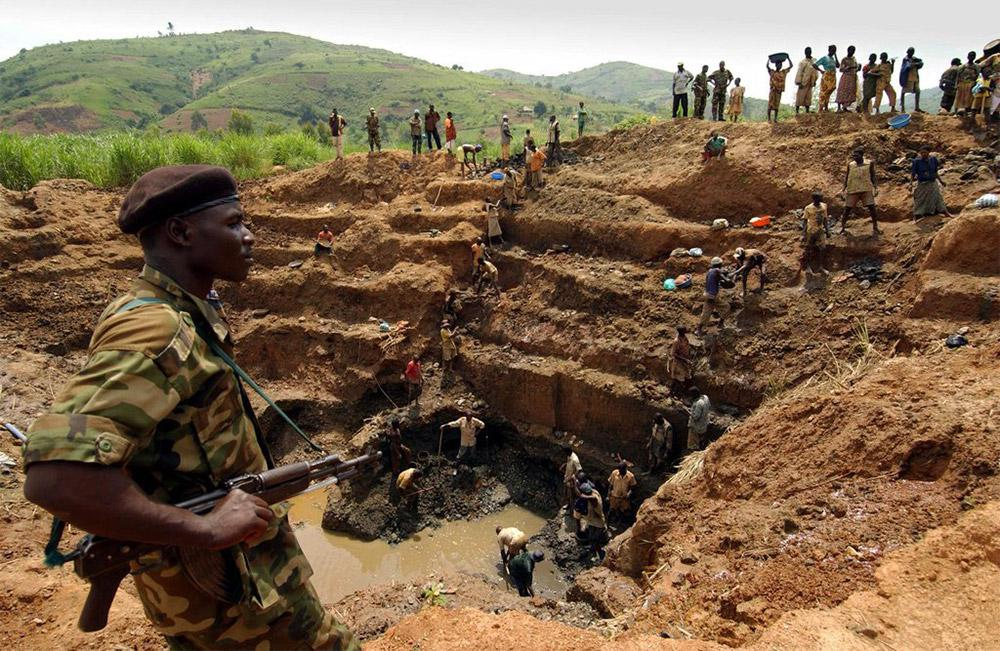
\includegraphics[width = 0.8\textwidth]{img/conflict_diamonds}

\vspace{10pt}
{\small Gold mine in Ituri region, eastern Democratic Republic of Congo (2003)}

\end{frame}
% ----------------------------------------------------

% ----------------------------------------------------
\begin{frame}
\frametitle{Greed \& opportunity}
\centering

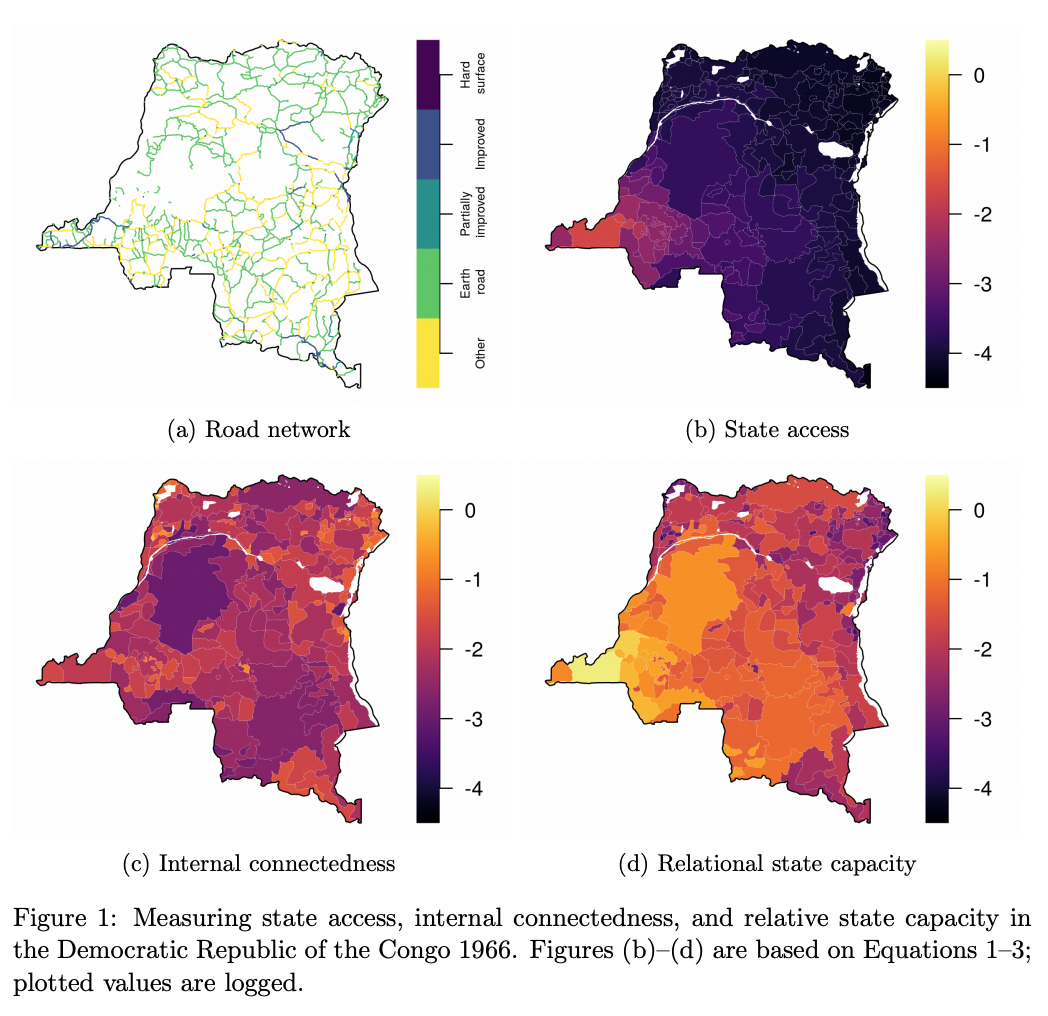
\includegraphics[width = 0.6\textwidth]{img/muller-crepon}

State capacity in the DRC in 1966\\
{\small (Müller-Crepon \textit{et al.}, 2020)}

\end{frame}
% ----------------------------------------------------

% ----------------------------------------------------
\begin{frame}
\frametitle{Greed \& opportunity: what they have in common}
\centering

\begin{itemize}[<+->]
  \item Ruling out \textit{motivational} factors related to ideology, religion, ethnicity, inequality...
  \item Previous explanations based on grievances do not work
  \item Grievances are ubiquitous, so they can't explain anything
  \item Empirical results: no effect of ethnic fractionalization
  \begin{itemize}
    \item Ethnic fractionalization: probability that two randomly drawn individuals belong to the same ethnic group (more ethnic groups, higher fractionalization)
  \end{itemize}
\end{itemize}

\end{frame}
% ----------------------------------------------------

% ----------------------------------------------------
\begin{frame}
\frametitle{What are grievances?}
\centering

\includegraphics[width = 0.6\textwidth]{img/revolt1381}

% {\small (English 1381 Peasants' Revolt)}
\begin{itemize}
  \item Outrage and historical rebellions
\end{itemize}

\end{frame}
% ----------------------------------------------------

% ----------------------------------------------------
\begin{frame}
\frametitle{What are grievances?}
\centering

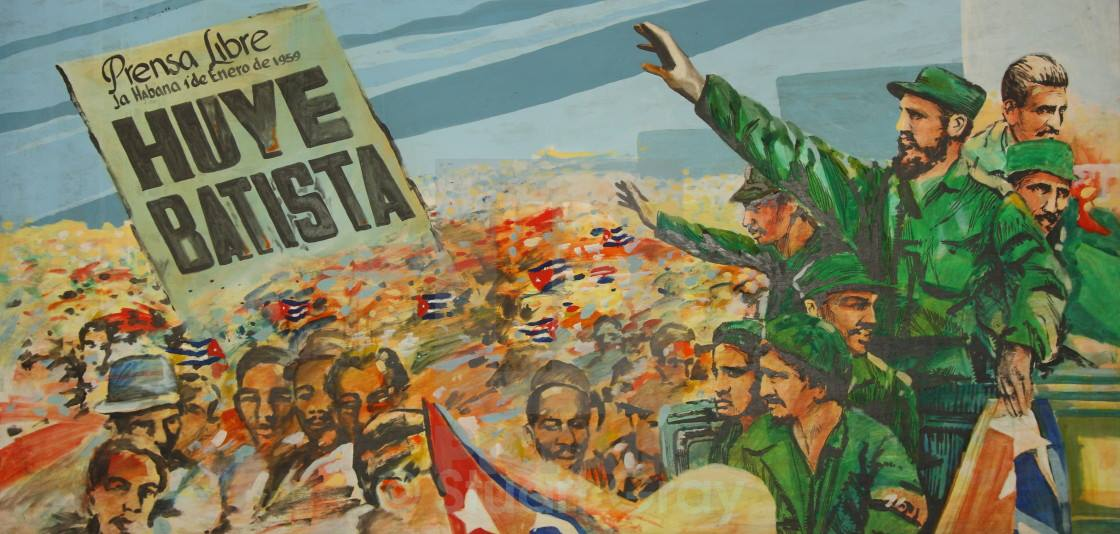
\includegraphics[width = \textwidth]{img/cuba}

\begin{itemize}
  \item Outrage and contemporary revolutions
\end{itemize}

\end{frame}
% ----------------------------------------------------

% ----------------------------------------------------
\begin{frame}
\frametitle{Grievances \& ideology in the greed perspective}
\centering

\begin{minipage}{0.55\textwidth}\centering
\begin{itemize}[<+->]
  \item Rebels `wrap' themselves in ideology
  \item But no real effect: we won't be able to predict the outbreak of civil wars based on the existence of grievances
  \item Is this true?
\end{itemize}
\end{minipage}\hfill
\begin{minipage}{0.44\textwidth}\centering
  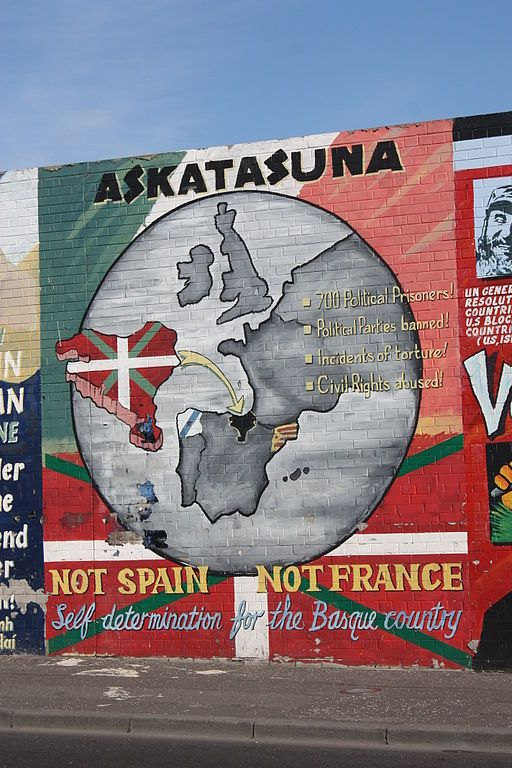
\includegraphics[width = 0.9\textwidth]{img/belfast_mural}

  {\small Mural in Belfast}
\end{minipage}

\end{frame}
% ----------------------------------------------------

% ----------------------------------------------------
\begin{frame}
\frametitle{The first wave of grievance studies}
\centering

\begin{minipage}{0.59\textwidth}\centering
\begin{itemize}[<+->]
  \item Context in the 60s: violence and revolution in the `Third World,' civil rights movement in the US
  \item What brings men and women to rise against `unjust' regimes?
  \item Focus on psychological mechanisms
  \item `Relative deprivation:' frustration over unmet expectations of material wellbeing triggers violent behavior
  \begin{itemize}
    \item In other words: `I'm not getting what I deserve'
  \end{itemize}
\end{itemize}
\end{minipage}\hfill
\begin{minipage}{0.4\textwidth}\centering
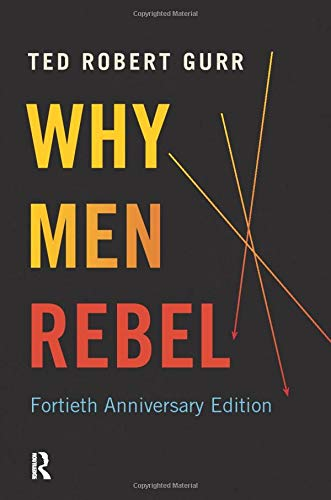
\includegraphics[width = 0.9\textwidth]{img/why_men_rebel}

Ted Gurr (1970)
\end{minipage}

\end{frame}
% ----------------------------------------------------

% ----------------------------------------------------
\begin{frame}
\frametitle{The first wave of grievance studies}
\centering

\begin{itemize}[<+->]
  \item Different from previous sociological theories of mob behavior, irrational mass behavior, etc
  \item Influenced by the ideological conflict of the Cold War
  \item Civil wars interpreted as `peasant revolutions' or `social revolutions'
\end{itemize}

\end{frame}
% ----------------------------------------------------

% ----------------------------------------------------
\begin{frame}
\frametitle{The first wave of grievance studies}
\centering

\begin{minipage}{0.59\textwidth}\centering
\begin{itemize}
  \item Rebellions in Burma, Cochinchina
  \item Subsistence economy, social reciprocity
  \item Traditional (feudal) moral economy that preserved subsistence, social preference for stability
  \item Market-based transformations destroy this moral equilibrium and breed rebellion
\end{itemize}
\end{minipage}\hfill
\begin{minipage}{0.4\textwidth}\centering
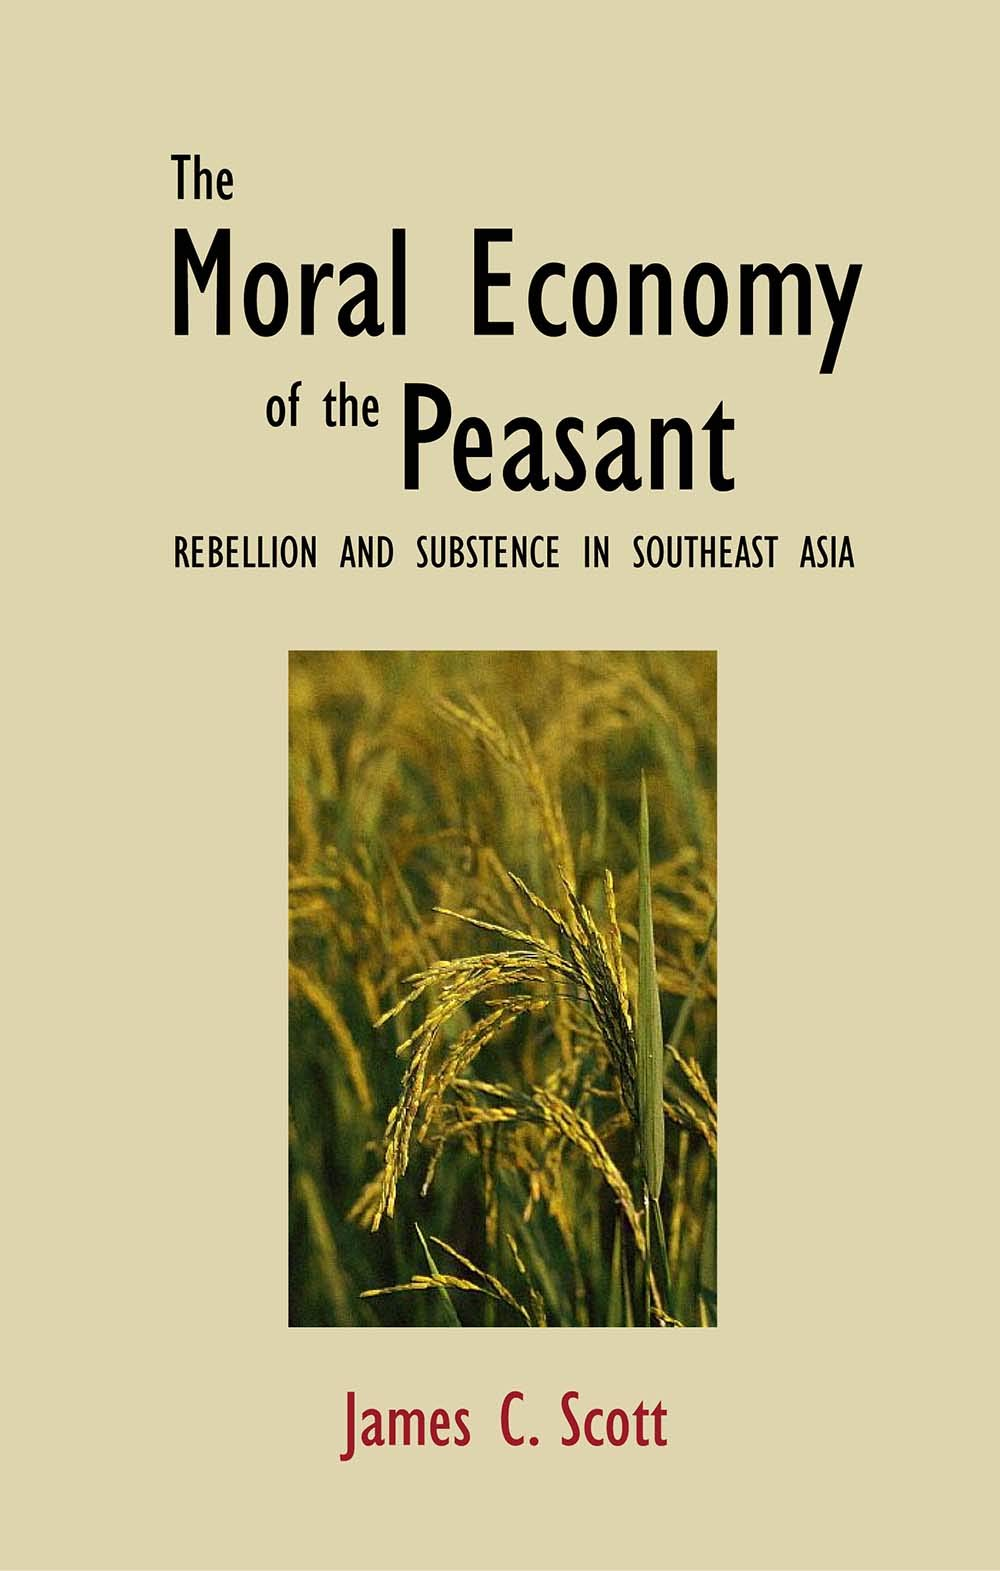
\includegraphics[width = 0.9\textwidth]{img/scott_moral}

James C Scott (1976)
\end{minipage}

\end{frame}
% ----------------------------------------------------

% ----------------------------------------------------
\begin{frame}
\frametitle{The first wave of grievance studies}
\centering

\begin{minipage}{0.59\textwidth}\centering
\begin{itemize}
  \item French, Russian, and Chinese Revolutions
  \item Social revolutions as a radical transformation of social and political structures (not a rebellion, not a political revolution)
  \item State-centric explanation of revolutions as a product of class struggle
\end{itemize}
\end{minipage}\hfill
\begin{minipage}{0.4\textwidth}\centering
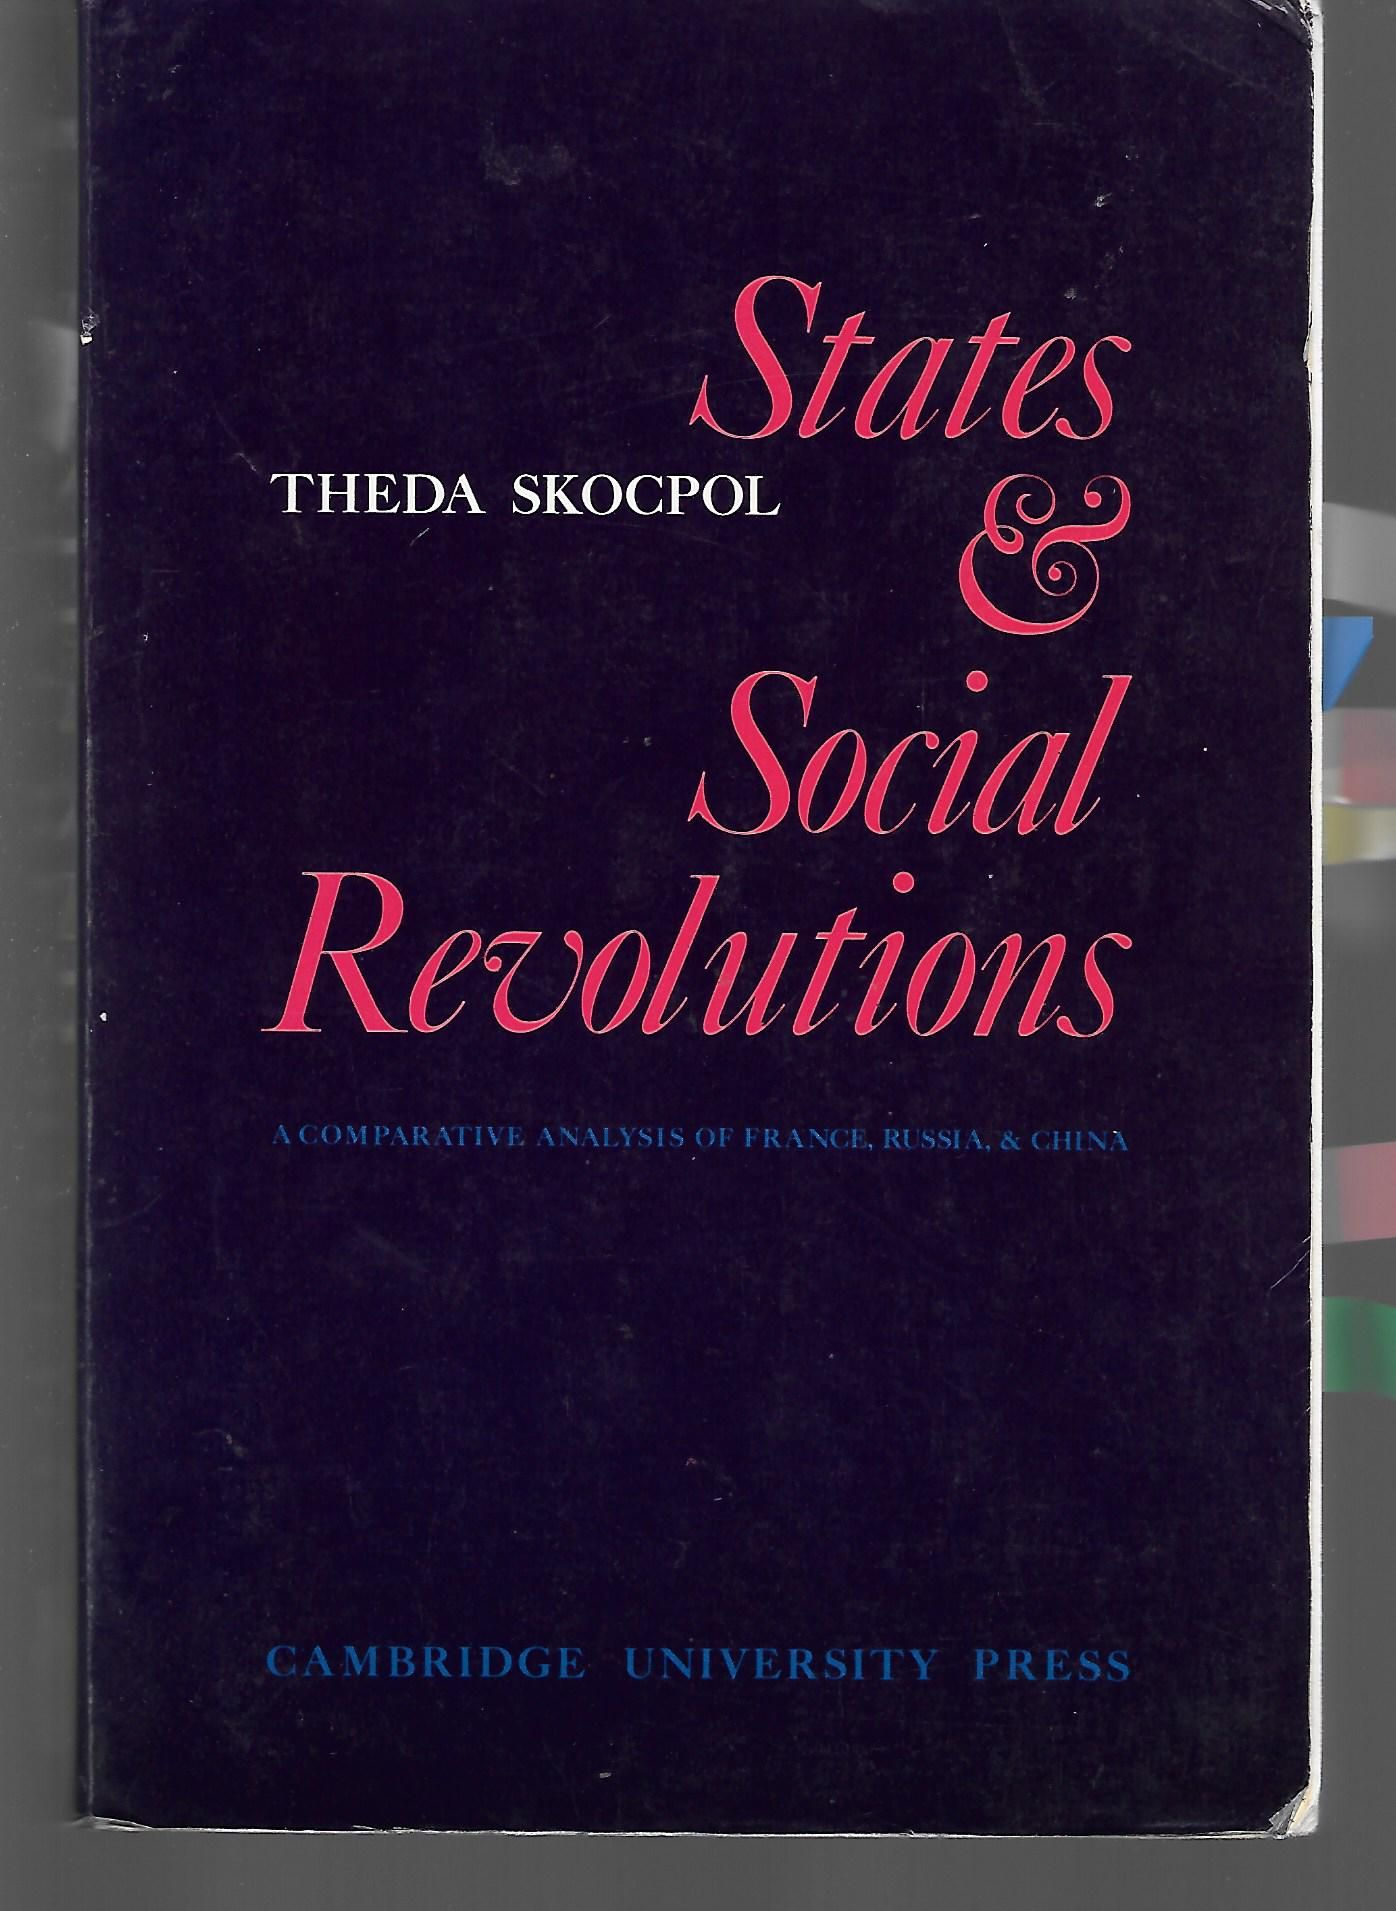
\includegraphics[width = 0.9\textwidth]{img/skocpol}

Theda Skocpol (1979)
\end{minipage}

\end{frame}
% ----------------------------------------------------

% ----------------------------------------------------
\begin{frame}
\frametitle{The first wave of grievance studies}
\centering

\begin{quote}
No social group is more conservative than a landowning peasantry and none is more revolutionary than a peasantry that owns too little land or pays too high a rental.
\end{quote}

\vspace{10pt}

{\footnotesize Samuel P Huntington (1968) \textit{Political Order in Changing Societies,} p. 375.}

\end{frame}
% ----------------------------------------------------

% ----------------------------------------------------
\begin{frame}
\frametitle{Early criticism or contributions}
\centering

\begin{itemize}[<+->]
  \item Collective action theory and the focus on opportunity structures (Tilly, \textit{From Mobilization to Revolution}): individual grievances or frustrations are not enough, resources and organization are needed for any form of collective action
  \item Rational action theory (Lichbach, \textit{The Rebel's Dilemma}): free riding problem, why would I individually contribute to the struggle?
  \item The role of culture and social groups (Michael Hechter, Donald Horowitz): not about frustrated individuals, but about group comparisons
\end{itemize}

\end{frame}
% ----------------------------------------------------

% ----------------------------------------------------
\begin{frame}
\frametitle{The new focus on ethnic groups in the 1990s}
\centering

\begin{itemize}[<+->]
  \item Lot of attention of a new set of conflicts where ethnic rivalries seems to play a huge role: Yugoslavia, Rwanda, former USSR, ongoing conflicts in Sri Lanka, Angola, ...
  \item Cold War perspective no longer present
  \item Posen's (1993) state collapse and ethnic security dilemma
  \item Primordialist accounts and ancient hatreds (Kaplan 1994)
  \item All this set the stage for the micro-economist approach and the greed/opportunity perspectives
\end{itemize}

\end{frame}
% ----------------------------------------------------

% ----------------------------------------------------
\begin{frame}
\frametitle{The new grievance perspective}
\centering

\begin{itemize}
  \item<1-> Critiques to grievances skepticism:
  \item<2-> Individualist approach and macro-level empirics
  \begin{itemize}
    \item Theories based on unitary individuals who seek material benefit
    \item But testing this with country-level measures that miss the point (e.g. ethnic fractionalization)
  \end{itemize}
  \item<3-> Structuralist approach and motivation
  \begin{itemize}
    \item Collective action theory and resource mobilization
    \item Why motivation based on material incentives but not on non-material ones?
  \end{itemize}
  \item<4-> Ethnic conflict and the state
  \begin{itemize}
    \item Where's the state in the ancient hatreds view?
    \item Ethnic conflict is usually \textit{about} controlling the state
  \end{itemize}
\end{itemize}

\end{frame}
% ----------------------------------------------------

% ----------------------------------------------------
\begin{frame}
\frametitle{The new grievance perspective}
\centering

\begin{minipage}{0.6\textwidth}\centering
  \begin{itemize}[<+->]
    \item Building on previous theories of grievances (Gurr) and social/ethnic groups (Horowitz, Hechter)
    \item Vertical and horizontal inequalities
    \begin{itemize}
      \item Inequalities not between individuals but between culturally defined groups
    \end{itemize}
    \item Nationalism and inequality
    \item Not captured by ethnic fractionalization, inequality measures (e.g. Gini), etc
  \end{itemize}
\end{minipage}\hfill
\begin{minipage}{0.39\textwidth}\centering
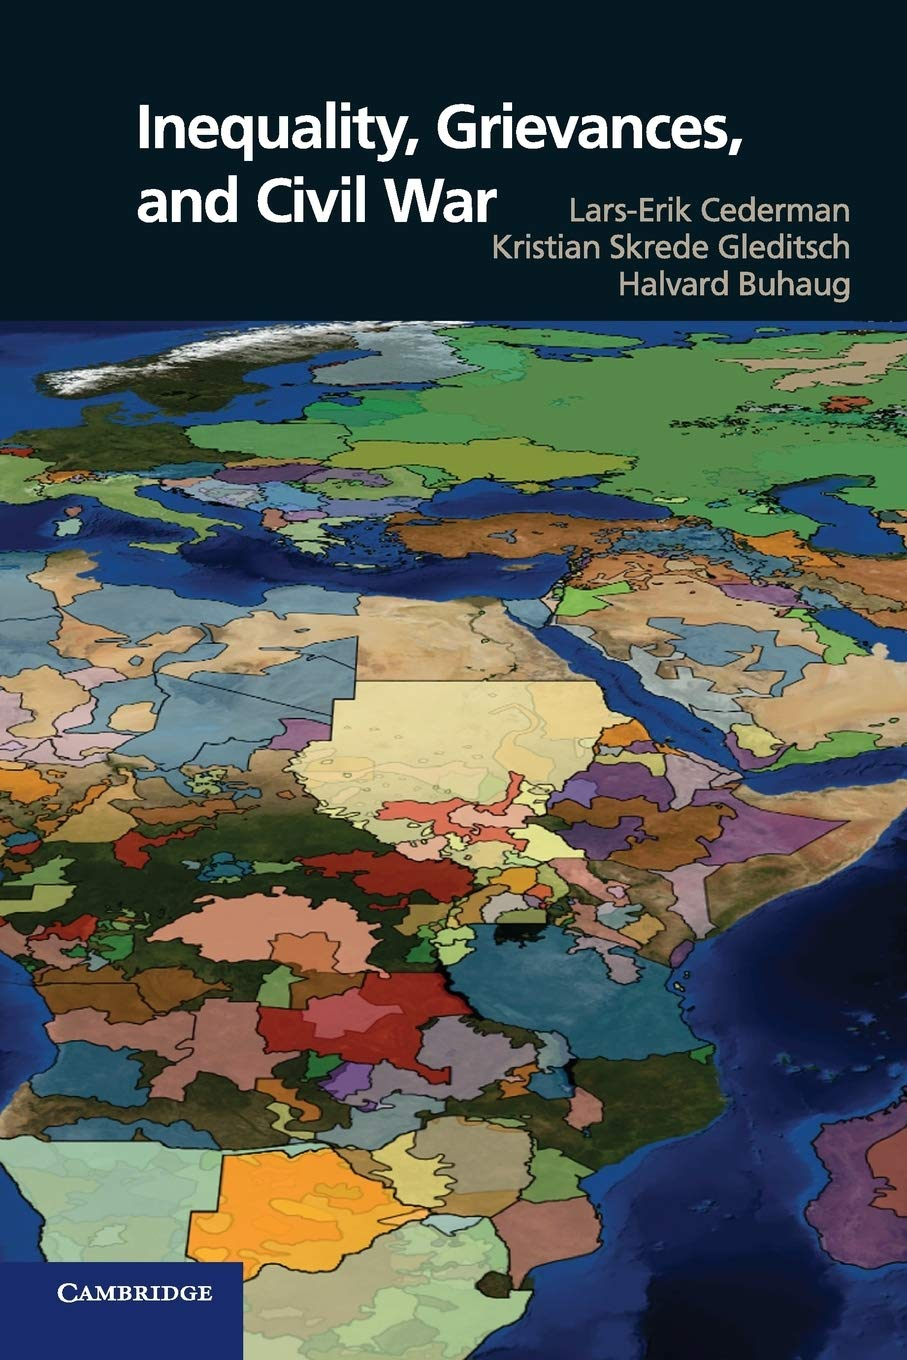
\includegraphics[width = 0.9\textwidth]{img/cgb}

{\small Cederman, Gleditsch, and Buhaug (2013)}
\end{minipage}

\end{frame}
% ----------------------------------------------------

% ----------------------------------------------------
\begin{frame}
\frametitle{From horizontal inequalities to conflict}
\centering

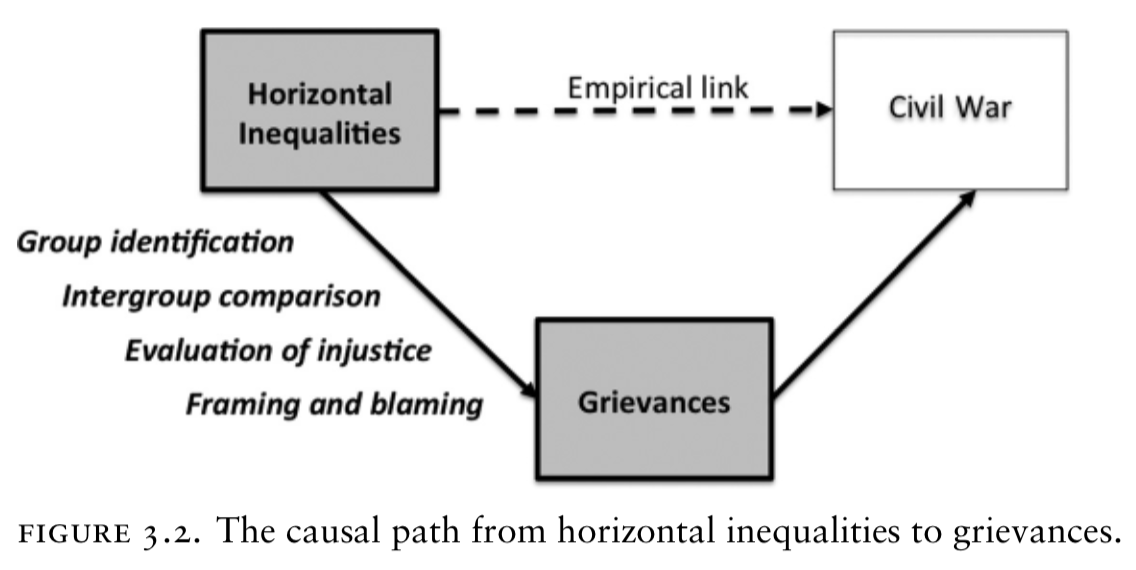
\includegraphics[width = 0.85\textwidth]{img/cgb_causal1}

\vspace{15pt}

{\small \textit{Source:} Cederman, Gleditsch, and Buhaug (2013)}

\end{frame}
% ----------------------------------------------------

% ----------------------------------------------------
\begin{frame}
\frametitle{From horizontal inequalities to conflict}
\centering

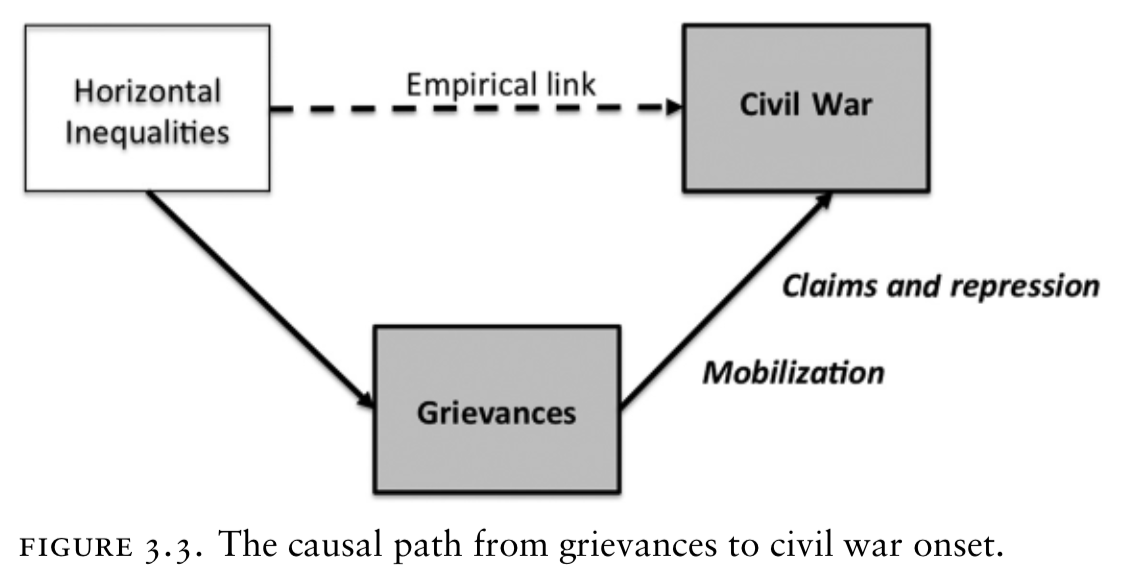
\includegraphics[width = 0.85\textwidth]{img/cgb_causal2}

\vspace{15pt}

{\small \textit{Source:} Cederman, Gleditsch, and Buhaug (2013)}

\end{frame}
% ----------------------------------------------------

% ----------------------------------------------------
\begin{frame}
\frametitle{Measuring grievances}
\centering

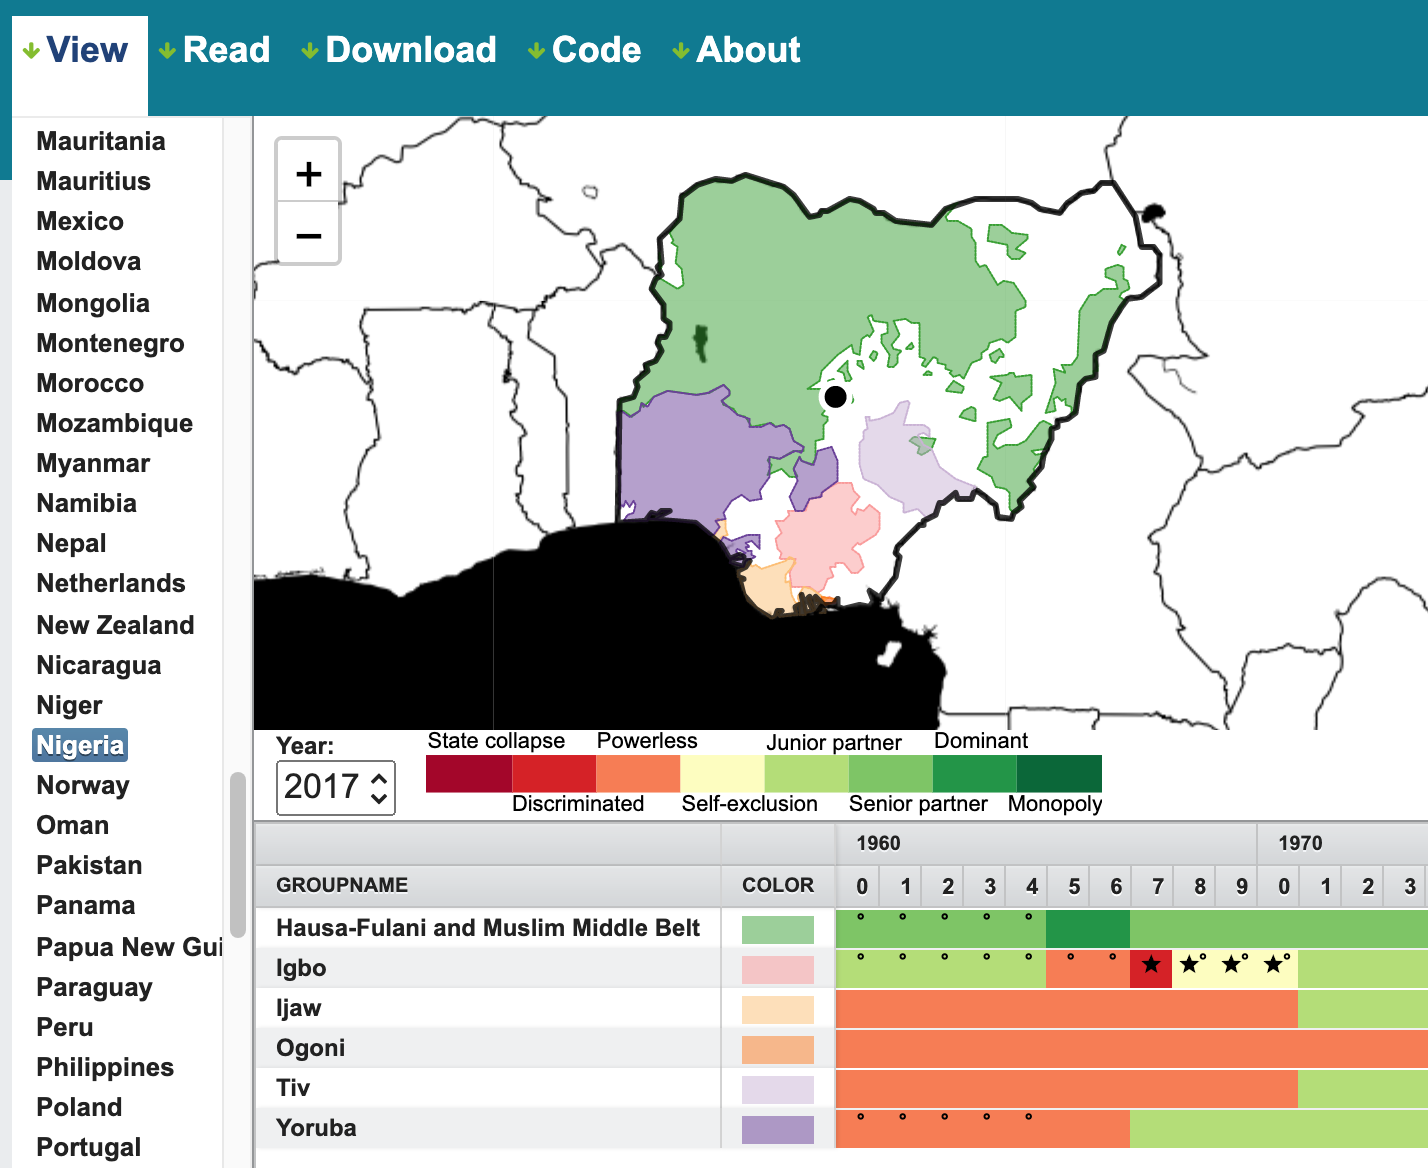
\includegraphics[width = 0.8\textwidth]{img/epr_nigeria}

\vspace{10pt}

{\small Ethnic Power Relations dataset (\url{https://growup.ethz.ch/})}

\end{frame}
% ----------------------------------------------------

% ----------------------------------------------------
\begin{frame}
\frametitle{Testing the effect of grievances}
\centering

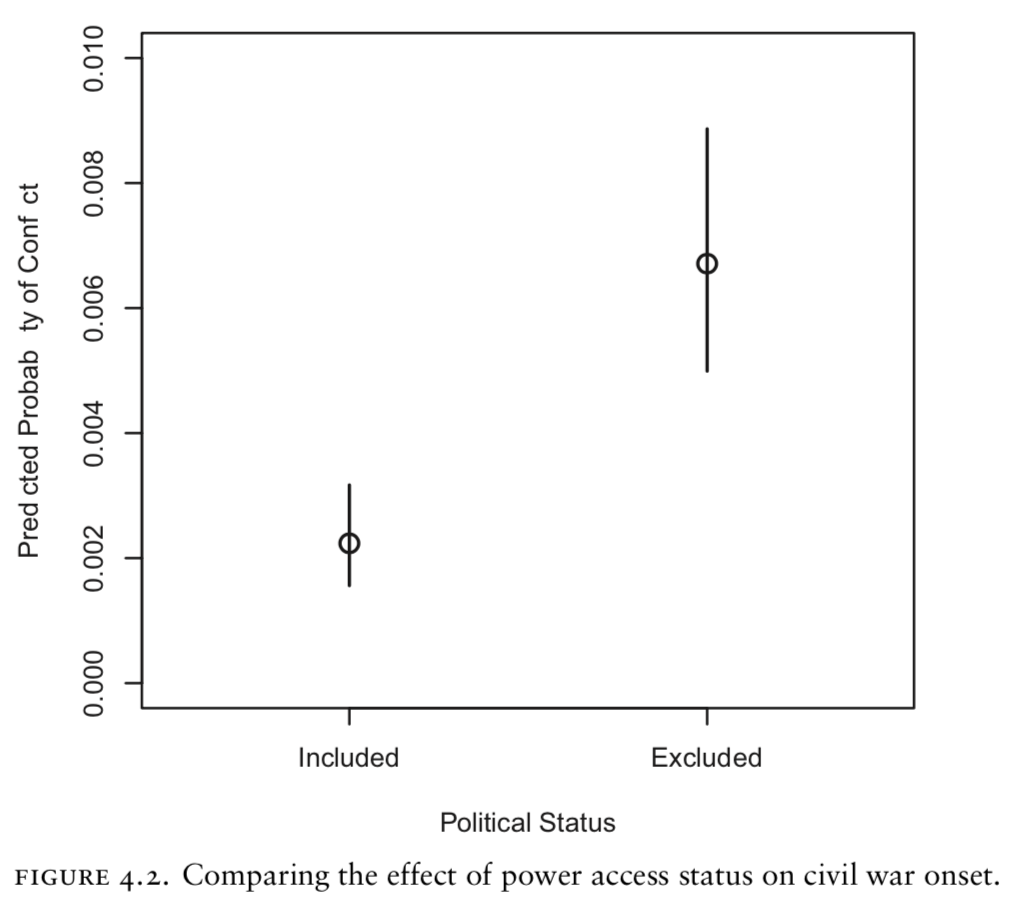
\includegraphics[width = 0.5\textwidth]{img/cgb_effect_exclusion}

\vspace{10pt}

{\small \textit{Source:} Cederman, Gleditsch, and Buhaug (2013)}

\vspace{15pt}

\begin{itemize}
  \item Being excluded from government linked to increased probability of conflict
\end{itemize}

\end{frame}
% ----------------------------------------------------

% ----------------------------------------------------
\begin{frame}
\frametitle{Testing the effect of grievances}
\centering

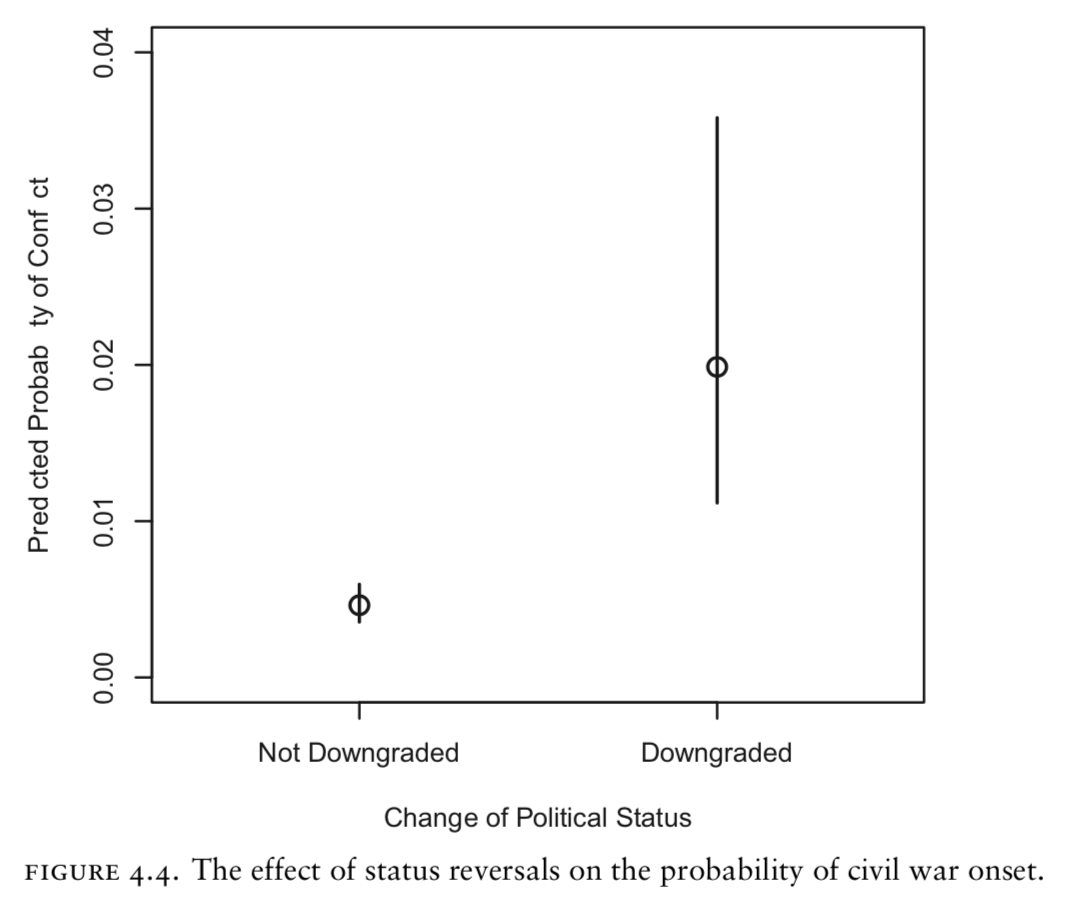
\includegraphics[width = 0.5\textwidth]{img/cgb_effect_downgrading}

\vspace{10pt}

{\small \textit{Source:} Cederman, Gleditsch, and Buhaug (2013)}

\vspace{15pt}

\begin{itemize}
  \item Losing status linked to increased probability of conflict
\end{itemize}

\end{frame}
% ----------------------------------------------------

% ----------------------------------------------------
\begin{frame}
\frametitle{The international system and the Cold War effect}
\centering

\begin{itemize}[<+->]
  \item Another take: Balcells \& Kalyvas (\textit{American Political Science Review}, 2010) and the international system
  \item How did global factors affected the \textit{technology of rebellion}?
  \item Remember the types:
  \begin{itemize}
    \item Irregular conflicts (guerrilla groups against conventional armies)
    \item Conventional civil wars (all conventional armies, clear frontlines)
    \item Symmetric non-conventional
  \end{itemize}
  \item Q: Did the change in the international system (end of Cold War) affect the way civil wars are fought?
\end{itemize}

\end{frame}
% ----------------------------------------------------

% ----------------------------------------------------
\begin{frame}
\frametitle{The Cold War effect (during \& after)}
\centering

\begin{itemize}[<+->]
  \item Main idea: superpower support in `proxy wars' increased insurgents' capacity, that's why we see so many irregular wars
  \item How? Material support, ideological support, training...
  \item Support to both sides
  \begin{itemize}
    \item E.g. the USSR supported the government of Mozambique and US supported RENAMO
  \end{itemize}
  \item After the Cold War, USSR support disappears and US no longer has incentives, and previously existing states collapse and armies fragment
  \item Increase in conventional and SNC wars
\end{itemize}

\end{frame}
% ----------------------------------------------------


% ----------------------------------------------------
\begin{frame}
\frametitle{The Cold War effect (during \& after)}
\centering

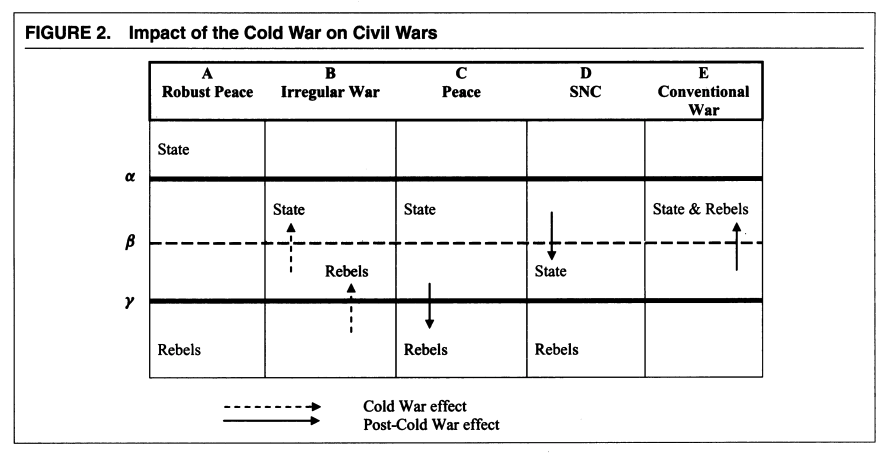
\includegraphics[width = 0.9\textwidth]{img/kalyvas_balcells_cold_war}

\begin{itemize}[<+->]
  \item Above $\alpha$: state is too strong (stable peace)
  \item Above $\beta$: able to use conventional armies
  \item Above $\gamma$: able to use irregular warfare
  \item Below $\gamma$: not enough military capacity (bandits, terrorists, etc)
\end{itemize}

\end{frame}
% ----------------------------------------------------

% ----------------------------------------------------
\begin{frame}
\frametitle{The golden age of the guerrillas}
\centering

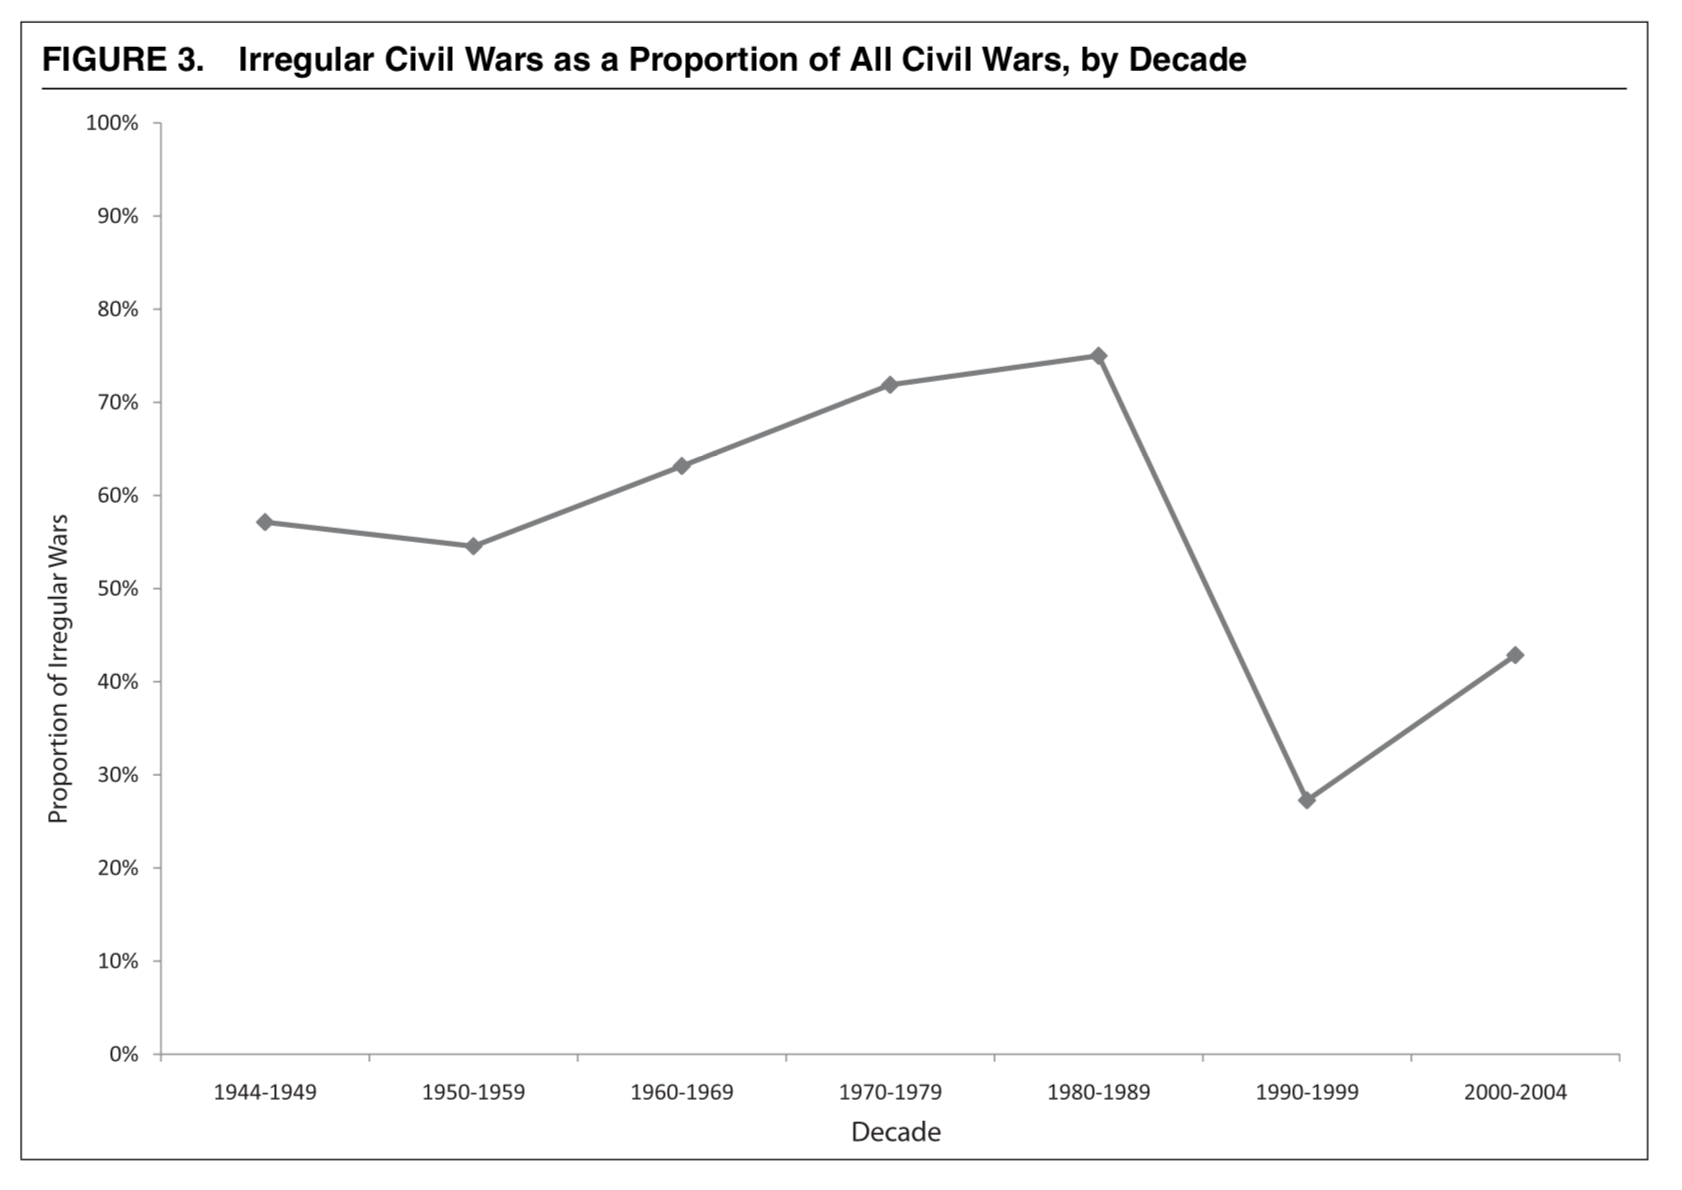
\includegraphics[width = \textwidth]{img/kalyvas_balcells_irr}

\end{frame}
% ----------------------------------------------------

% ----------------------------------------------------
\begin{frame}
\frametitle{The golden age of the guerrillas}
\centering

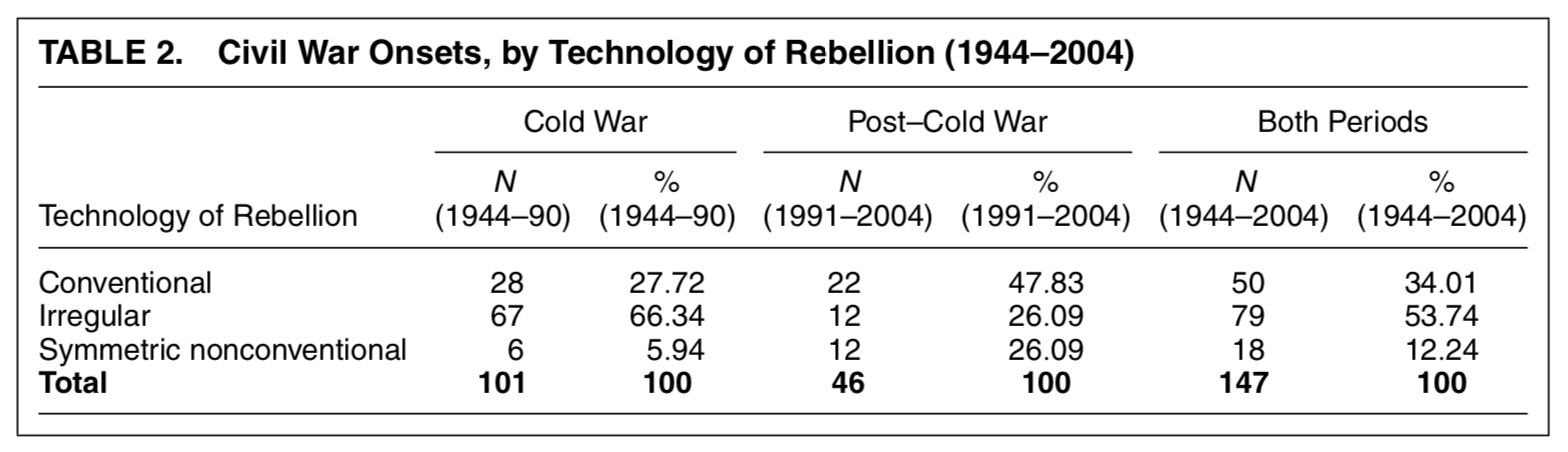
\includegraphics[width = \textwidth]{img/kalyvas_balcells_table}

\end{frame}
% ----------------------------------------------------

% ----------------------------------------------------
\begin{frame}
\frametitle{Wrapping up: explaining why civil wars break out}
\centering

\begin{itemize}
  \item<1-> Two key perspectives in academic research and policy-making
  \item<2-> Greed (or opportunity)
    \begin{itemize}
      \item Highlighting the opportunities of insurgencies to launch an insurgency
      \item Economic and rational analysis of war onset
      \item Dismissing motivational factors (ethnicity, discrimination, religion, etc)
    \end{itemize}
  \item<3-> Grievance (or motivation)
  \begin{itemize}
    \item Role of horizontal inequalities
    \item Critique to F\&L: empirical measures do not reflect this (ethnic fractionalization)
  \end{itemize}
\end{itemize}

\end{frame}
% ----------------------------------------------------

% ----------------------------------------------------
\begin{frame}
\frametitle{Beyond greed vs grievance}
\centering

\begin{itemize}[<+->]
  \item No perspective (greed, grievances, opportunity) is sufficient to explain civil wars \textit{on its own}
  \item Recent research (and policy) focuses on combining them, for instance:
  \begin{itemize}
    \item Grievances can complement resource-based models of collective action
    \item State capacity is probably the most important factor, but also includes a cultural aspect (nation-building)
    \item Opportunistic or \textit{greedy} leaders can co-exist with ideology-motivated participants
  \end{itemize}
  \item Alternative points of view: e.g., the role of the international system
\end{itemize}

\end{frame}
% ----------------------------------------------------

% ----------------------------------------------------
\begin{frame}
\frametitle{Beyond conflict onset}
\centering

\begin{itemize}[<+->]
  \item Main focus is on civil war onset, which roughly tries to explain why at some point individuals decide to use organized violence against the state
  \item But if we care about civil wars because of the human suffering (or even economic consequences), we should look at least at two different things
  \begin{itemize}
    \item How long do wars last?
    \item Why do wars break out again? (we'll see this in the postwar week)
  \end{itemize}
\end{itemize}

\end{frame}
% ----------------------------------------------------

% ----------------------------------------------------
\begin{frame}
\frametitle{Looking at the \textit{duration} of civil wars}
\centering

\begin{itemize}[<+->]
  \item Fearon (2004) `Why do some civil wars last so much longer than others?'
  \item Two types of particularly long conflicts:
  \begin{itemize}
    \item Conflicts where rebel groups receive funding from contraband activities: diamonds, coca, opium...
    \item `Sons-of-the-soil' conflicts: ethnic minority in the periphery against a dominant ethnic group that supports migrants into the periphery
  \end{itemize}
  \item Commitment problems
  \begin{itemize}
    \item Why would I stop fighting and reach a negotiated settlement?
    \item Wartime contraband is making me rich even if fighting is costly
    \item I'm sending migrants of my group to your region, which will increase in local power in the future
  \end{itemize}
\end{itemize}
% Balcells, L., & Kalyvas, S. N. (2014). Does Warfare Matter? Severity, Duration, and Outcomes of Civil Wars. Journal of Conflict Resolution, 58(8), 1390–1418.

\end{frame}
% ----------------------------------------------------

% ----------------------------------------------------
\begin{frame}
\frametitle{Looking at the \textit{duration} of civil wars}
\centering

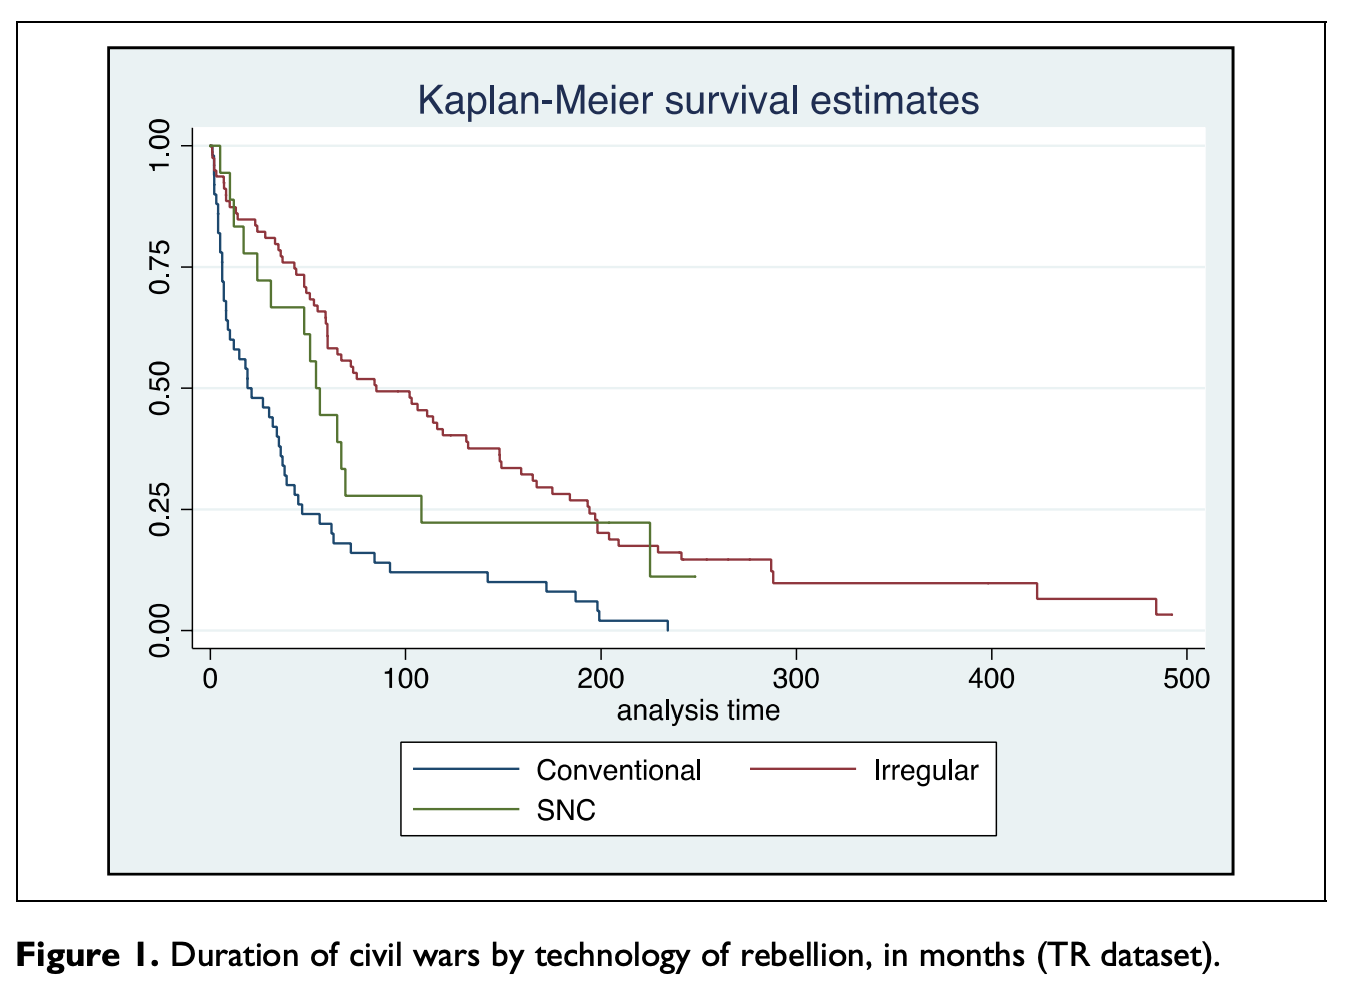
\includegraphics[width = 0.8\textwidth]{img/balcells_kalyvas_duration}

% \vspace{10pt}

\begin{itemize}
  \item Balcells \& Kalyvas (\textit{Journal of Conflict Resolution,} 2014)
  \item Looking at the duration depending on technology of rebellion
\end{itemize}

% Balcells, L., & Kalyvas, S. N. (2014). Does Warfare Matter? Severity, Duration, and Outcomes of Civil Wars. Journal of Conflict Resolution, 58(8), 1390–1418.

\end{frame}
% ----------------------------------------------------





% ----------------------------------------------------
\begin{frame}
\frametitle{Next seminar #1}
\centering

\begin{minipage}{0.55\textwidth}\centering
\begin{itemize}
  \item Robert D Kaplan, `The coming anarchy' (\textit{The Atlantic,} 1994)
  \item Pessimist view on Post-Cold War international security
\end{itemize}
\end{minipage}\hfill
\begin{minipage}{0.44\textwidth}\centering
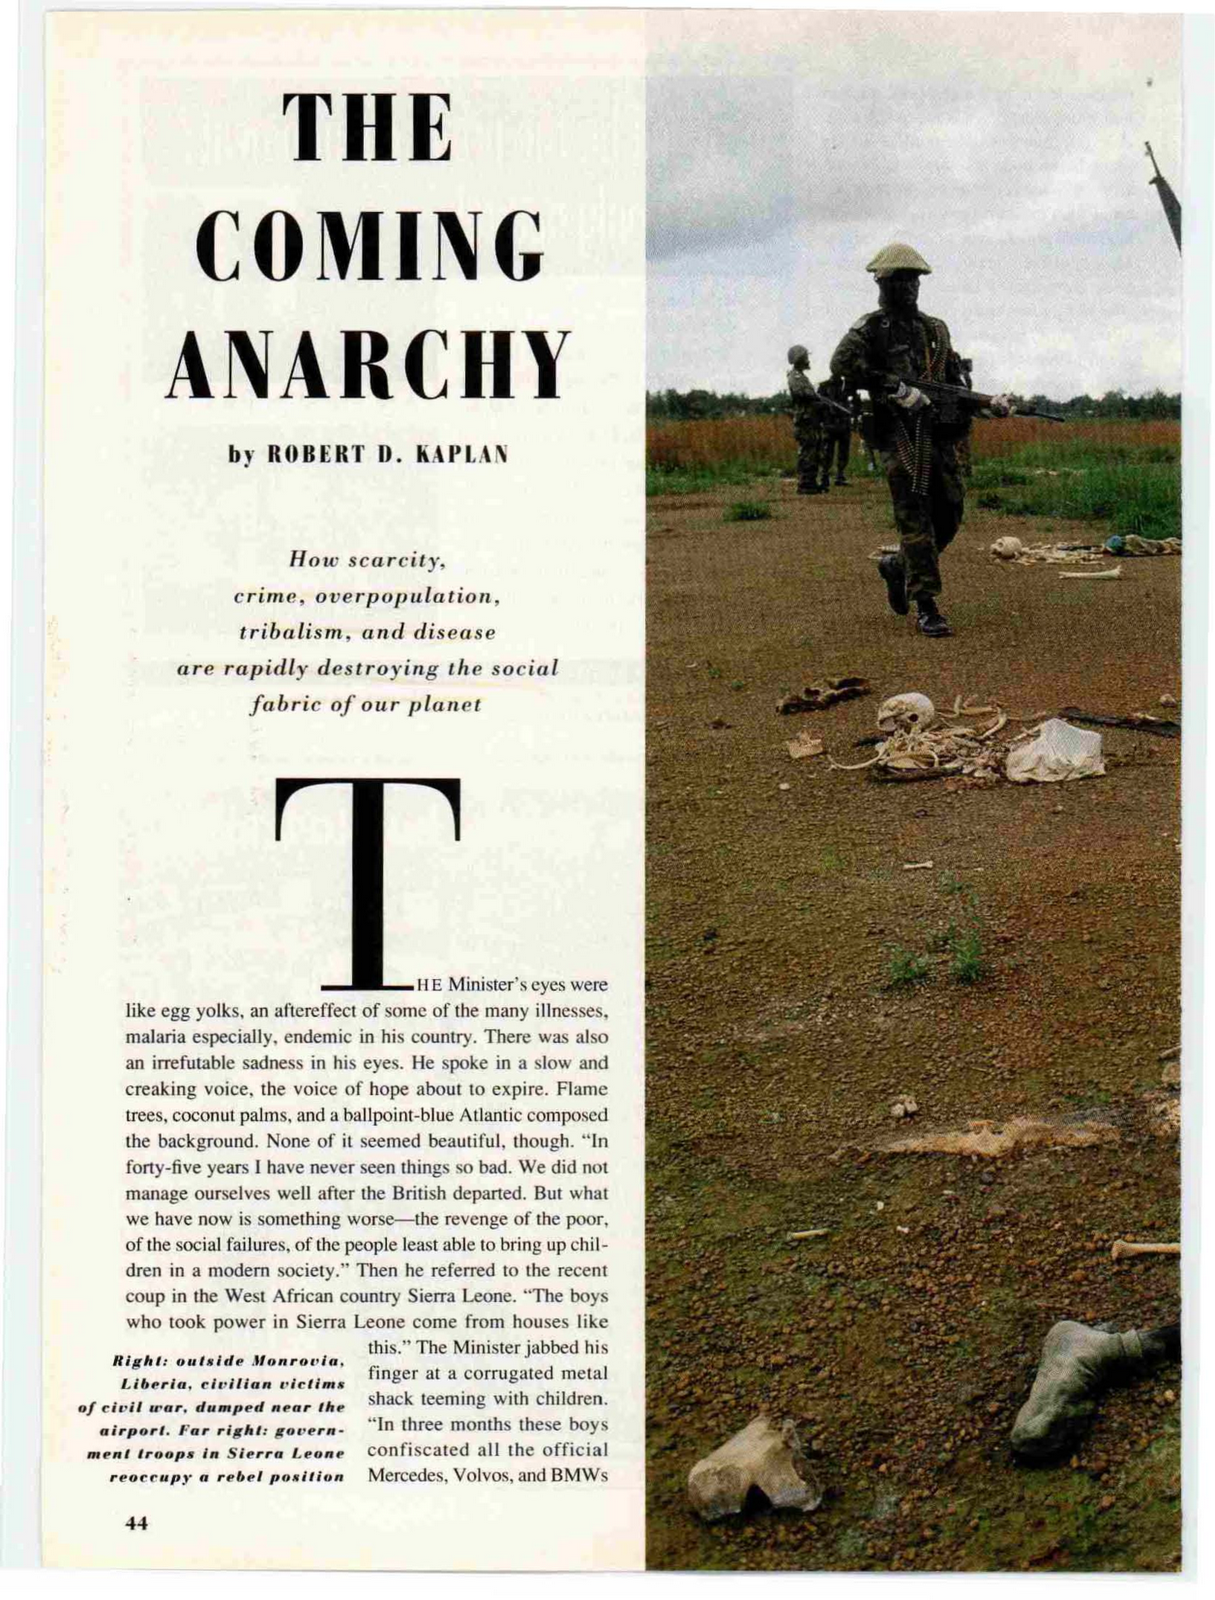
\includegraphics[width = \textwidth]{img/ComingAnarchy}
\end{minipage}

\end{frame}
% ----------------------------------------------------

% ----------------------------------------------------
\begin{frame}
\frametitle{Next seminar #2}
\centering

\begin{minipage}{0.55\textwidth}\centering
\begin{itemize}
  \item Anand Gopal, `The other Afghan women' (\textit{New Yorker,} Sept 2021)
  \item Why women turned against the US and supported the Taliban
\end{itemize}
\end{minipage}\hfill
\begin{minipage}{0.44\textwidth}\centering
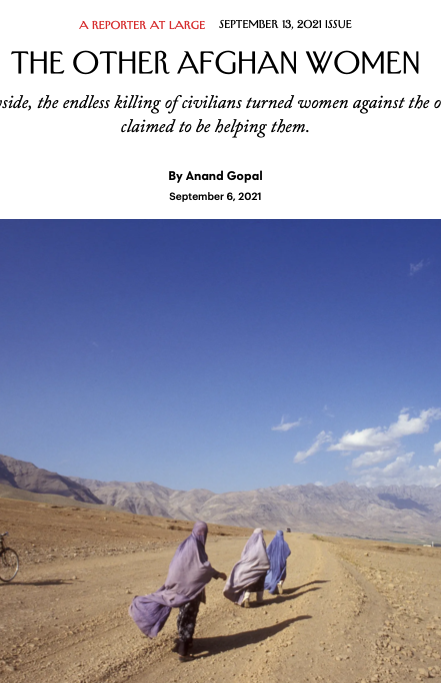
\includegraphics[width = \textwidth]{img/gopal}
\end{minipage}

\end{frame}
% ----------------------------------------------------

\end{document}
